\documentclass[fleqn,addpoints]{exam}

\usepackage{graphicx}
\usepackage{float}
\usepackage{amsmath}
\usepackage{cancel}
\usepackage{polynom}
\usepackage{caption}

\printanswers

\ifprintanswers 
% \usepackage{2in1, lscape} 
\fi

\title{Math 115 Homework 13}
\date{January 11, 2011}

\begin{document}

\maketitle
 
\ifprintanswers
\else
\section{Administrative}
We won't have class on 1/18 because the PAB will be closed.  If everyone is available, we'll meet during study
hall in the morning of 1/15 instead.  We'll talk about section 2.5 from DeFranza and review for the test.

The Chapter 2 exam will be on 1/25.

\section{Reading}
\begin{itemize}
  \item Larson/Hostetler Section 2.6
  \item Faires/DeFranza Section 2.4
\end{itemize}

\section{Homework}

This homework is due on 1/25 since we won't have class on 1/18.

\begin{itemize}
  \item Larson/Hostetler, pp 267: 15-20, 25-26, 29-31, 35-36, 39-40, 44, 53, 55-56, 61-62, 71, 73
\end{itemize}

You'll probably want to use a calculator (it doesn't need to be a graphing calculator) on problems 71 and 73.  If you
can't get to a calculator, you can still answer the limit parts of the questions.

\fi

\ifprintanswers

\section{Larson/Hostetler}

\begin{description}
\item[25]
\begin{figure}[H]
  \centering
  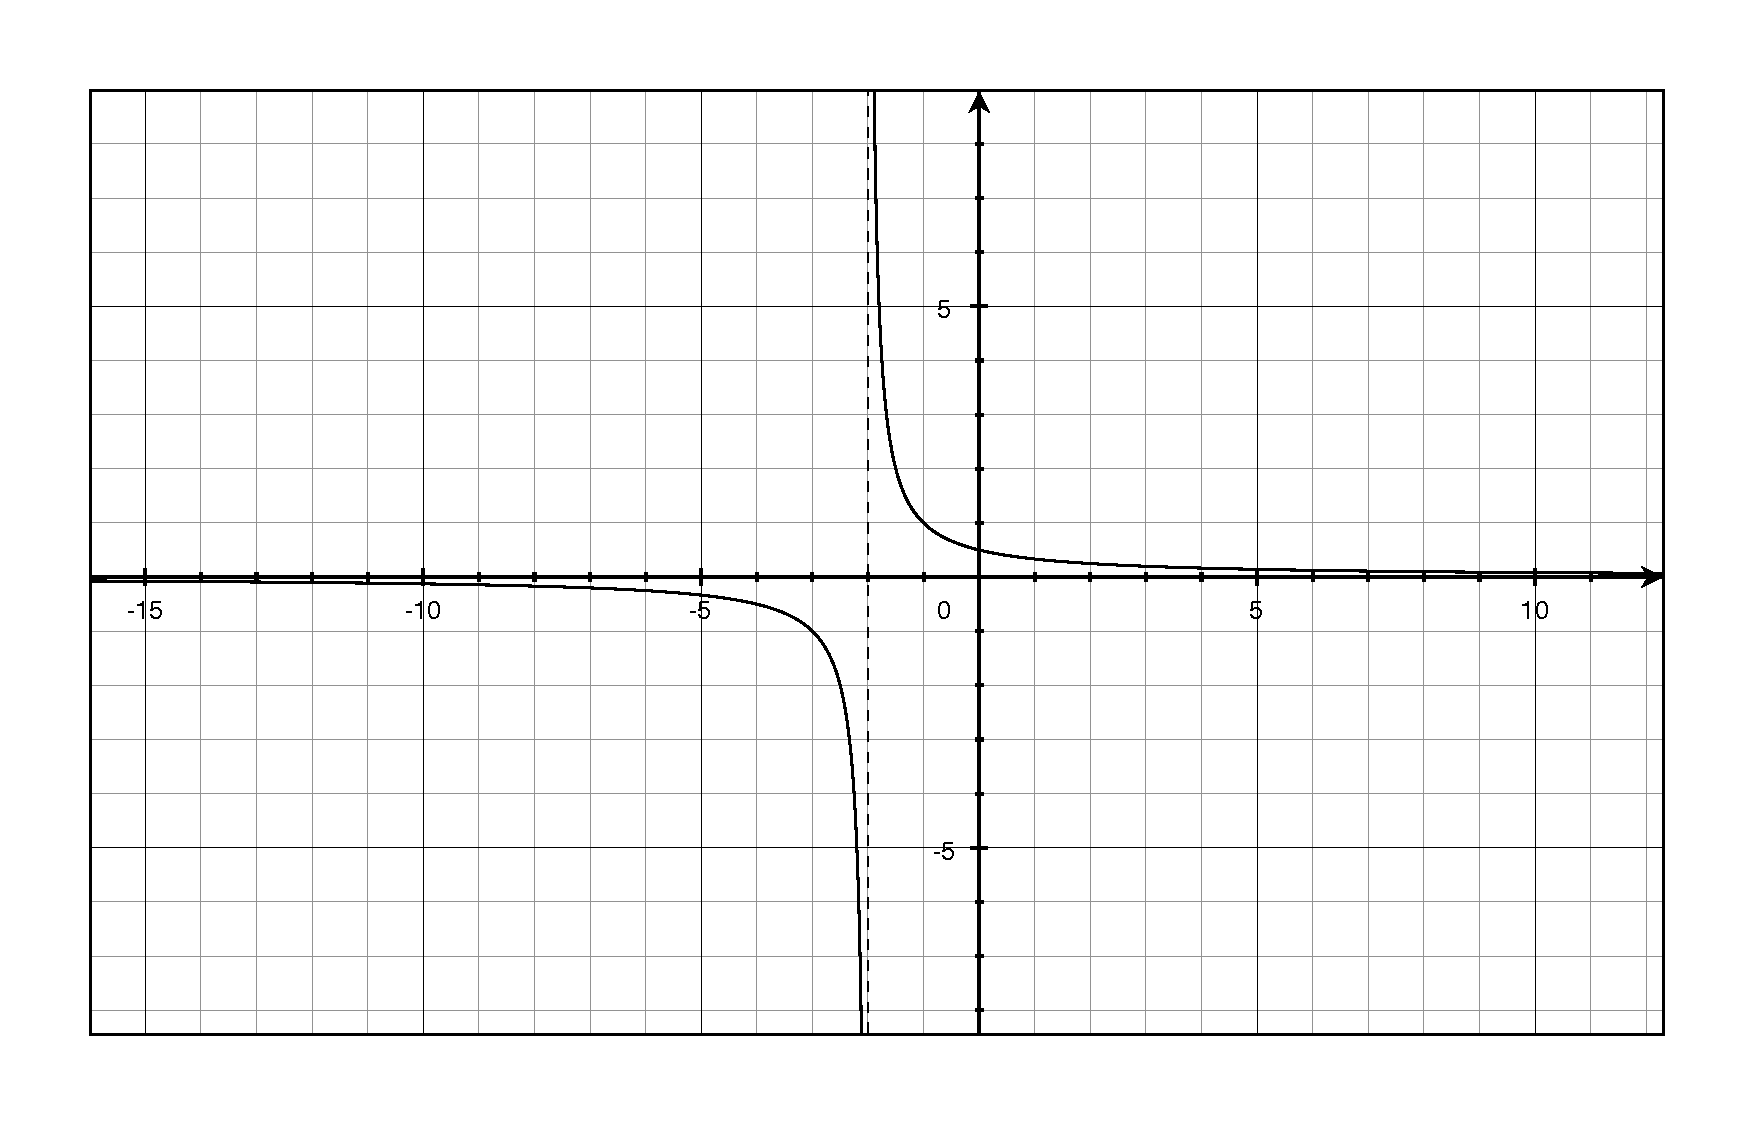
\includegraphics[width=12.25cm,height=8.75cm]{question25.eps}
  \caption*{Question 25}
\end{figure}

\item[26]
\begin{figure}[H]
  \centering
  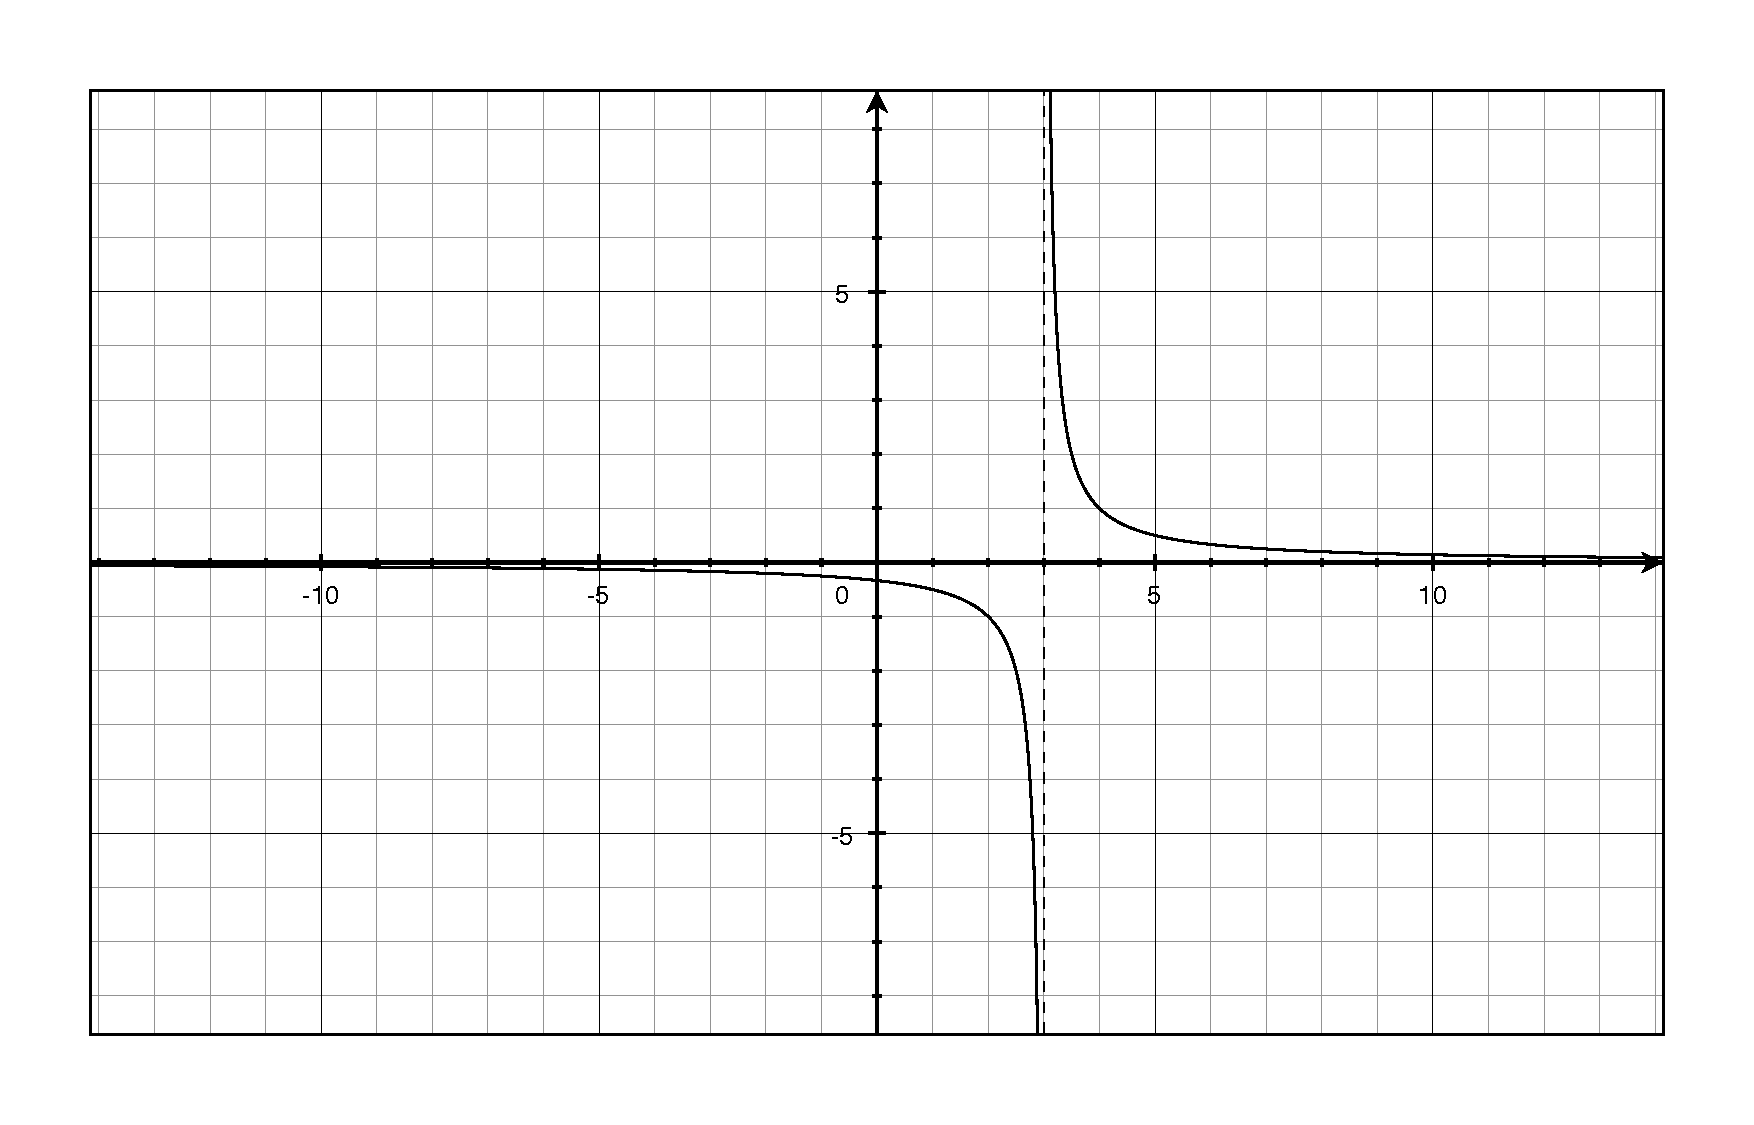
\includegraphics[width=12.25cm,height=8.75cm]{question26.eps}
  \caption*{Question 26}
\end{figure}

\item[29]
\begin{figure}[H]
  \centering
  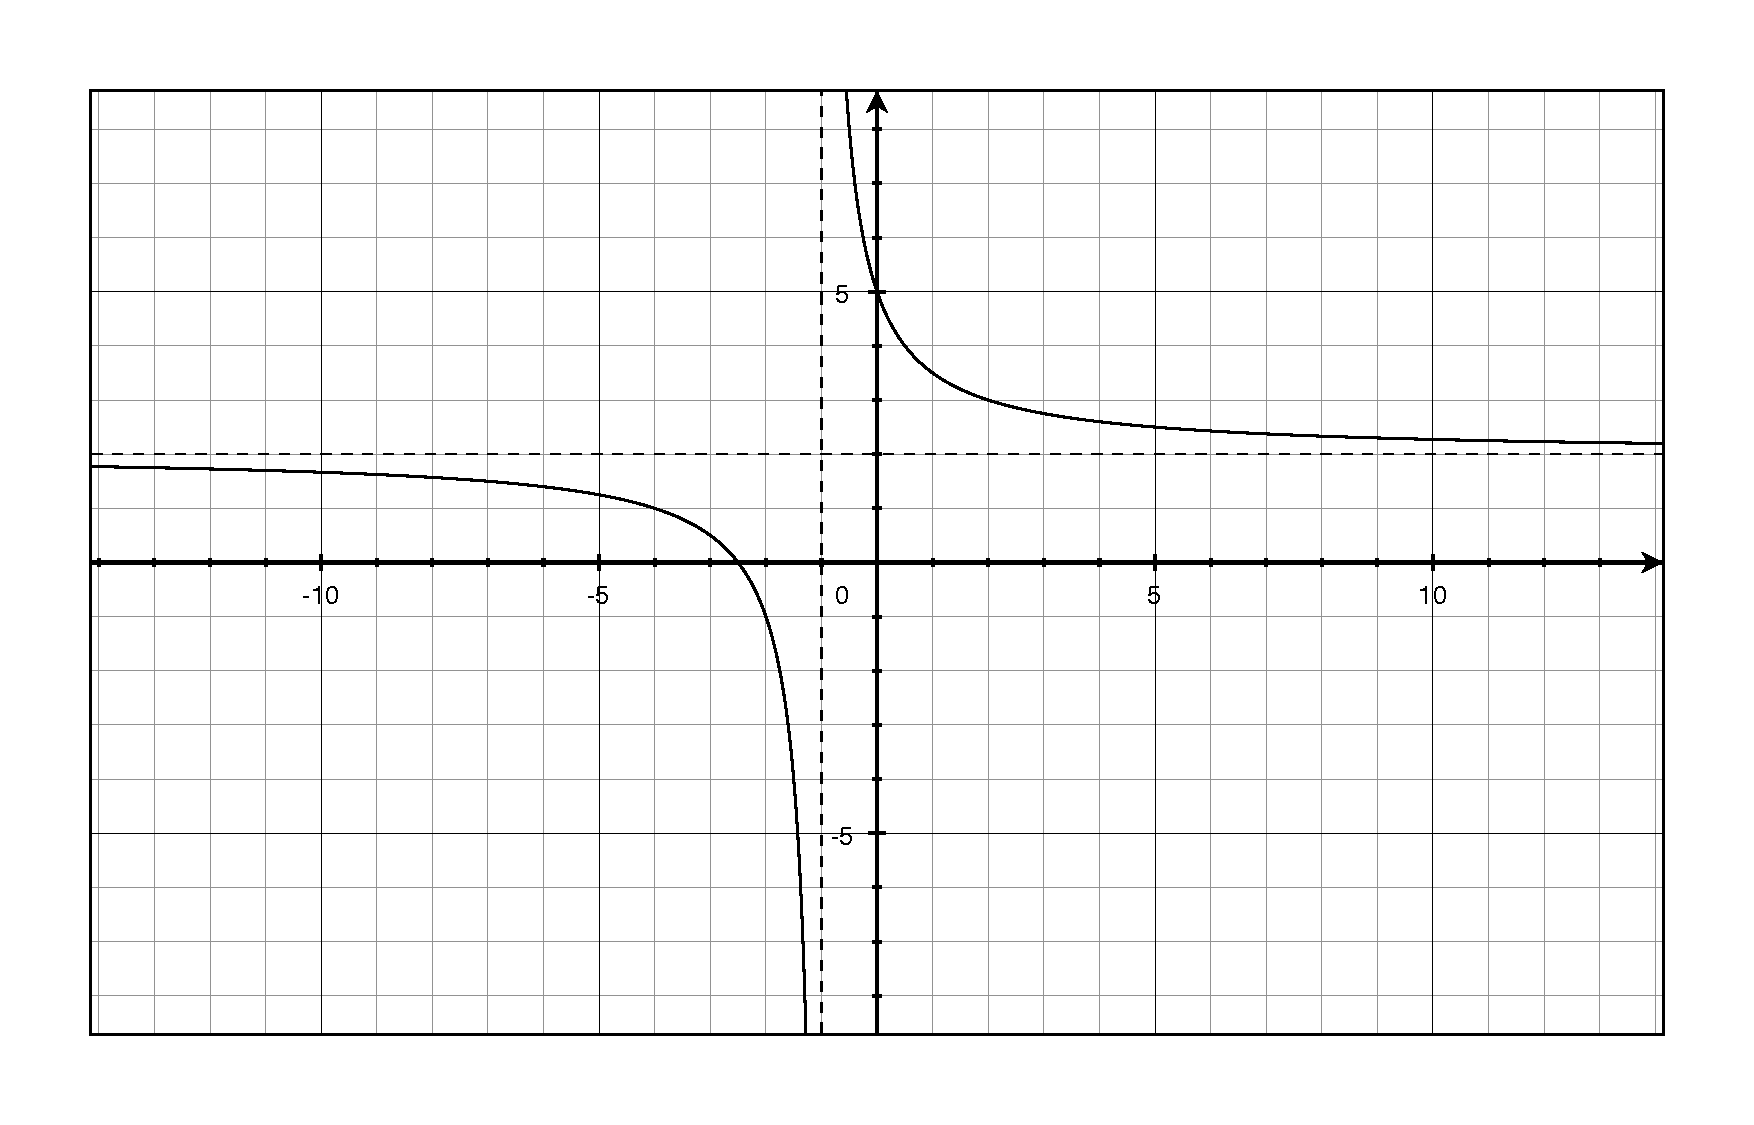
\includegraphics[width=12.25cm,height=8.75cm]{question29.eps}
  \caption*{Question 29}
\end{figure}

\item[30]
\begin{figure}[H]
  \centering
  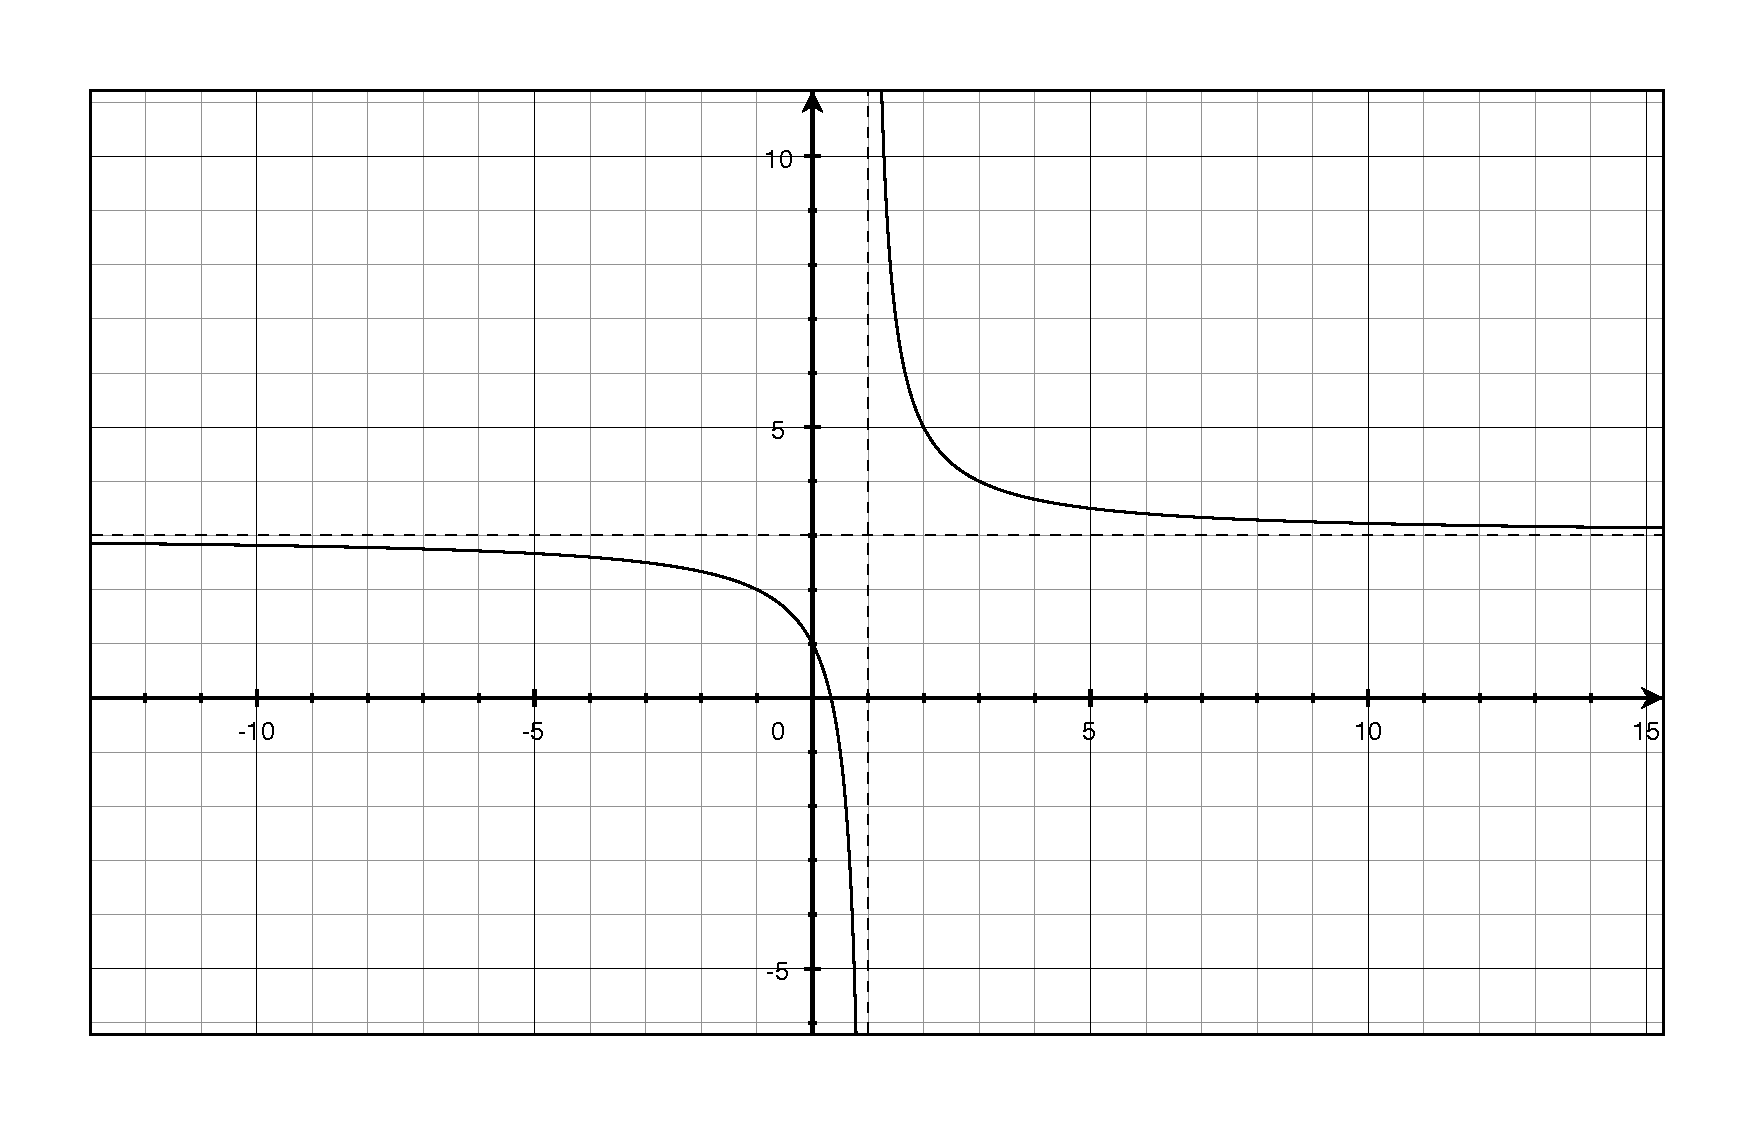
\includegraphics[width=12.25cm,height=8.75cm]{question30.eps}
  \caption*{Question 30}
\end{figure}

\item[31]
\begin{figure}[H]
  \centering
  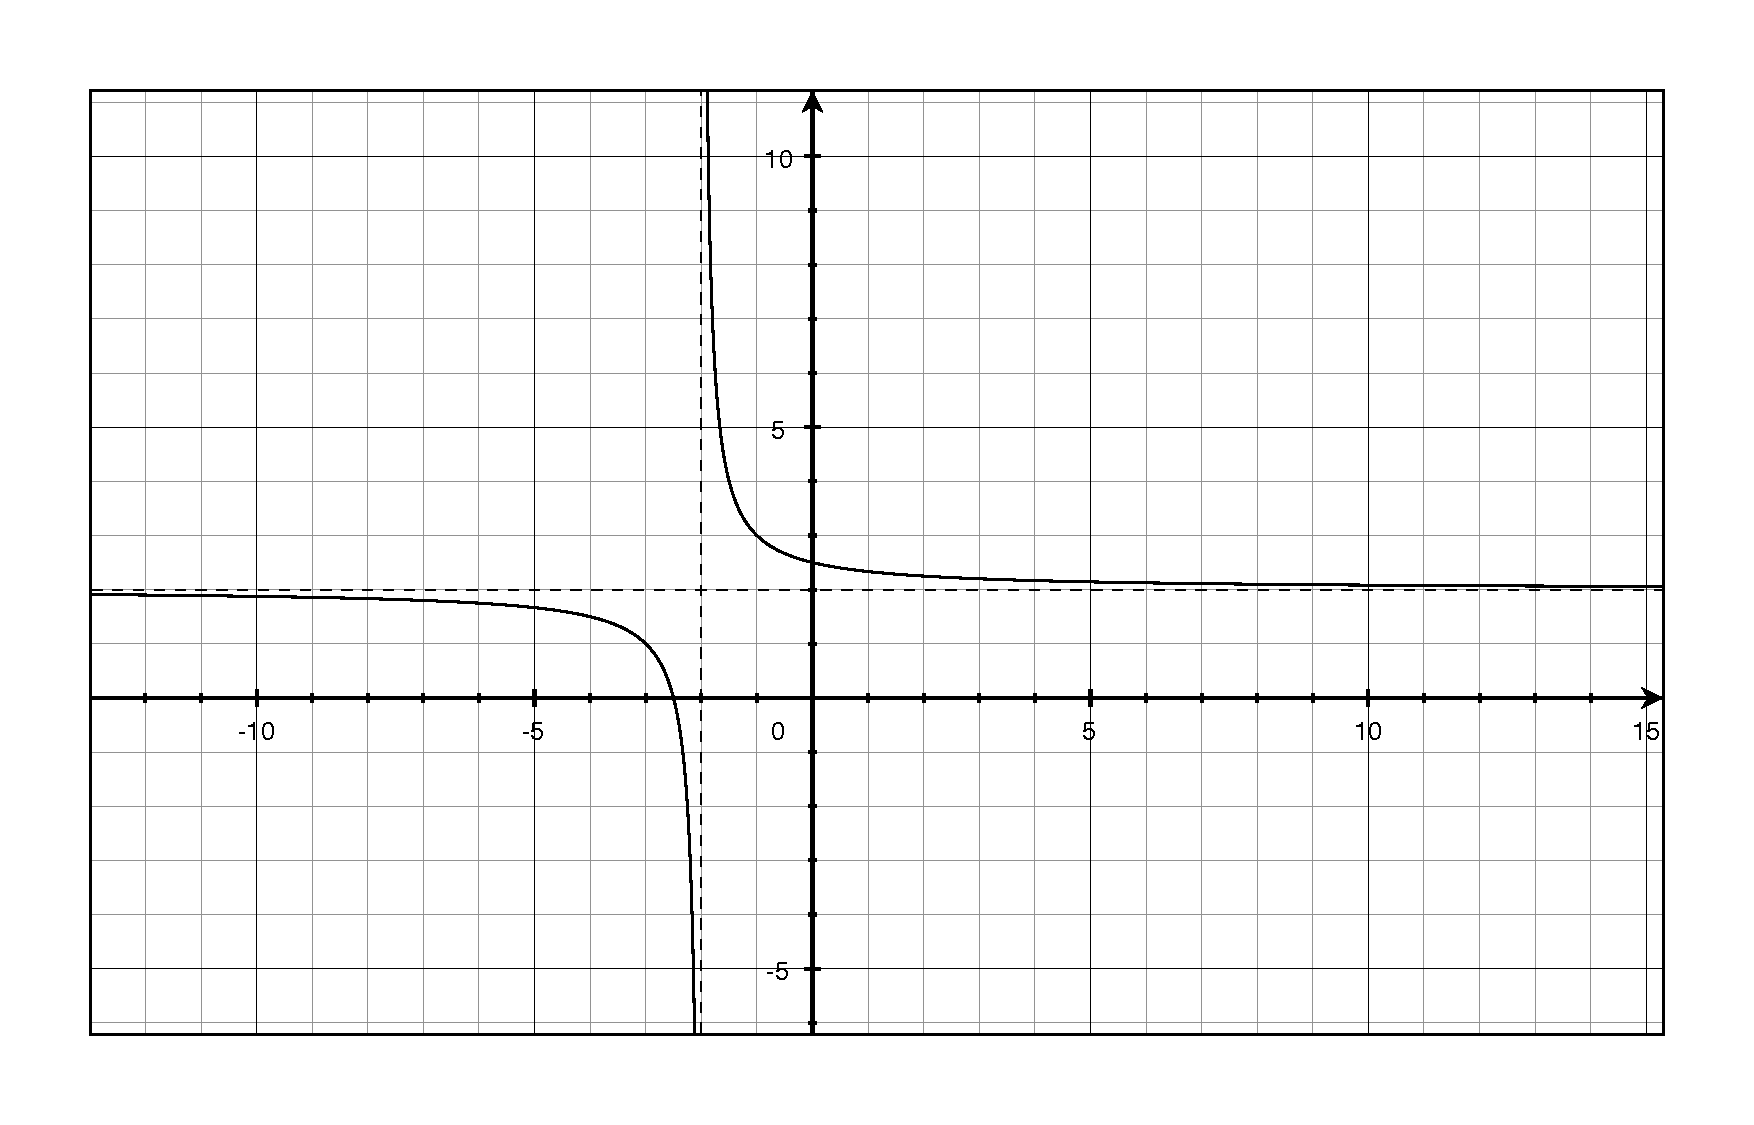
\includegraphics[width=12.25cm,height=8.75cm]{question31.eps}
  \caption*{Question 31}
\end{figure}

\item[35]
\begin{figure}[H]
  \centering
  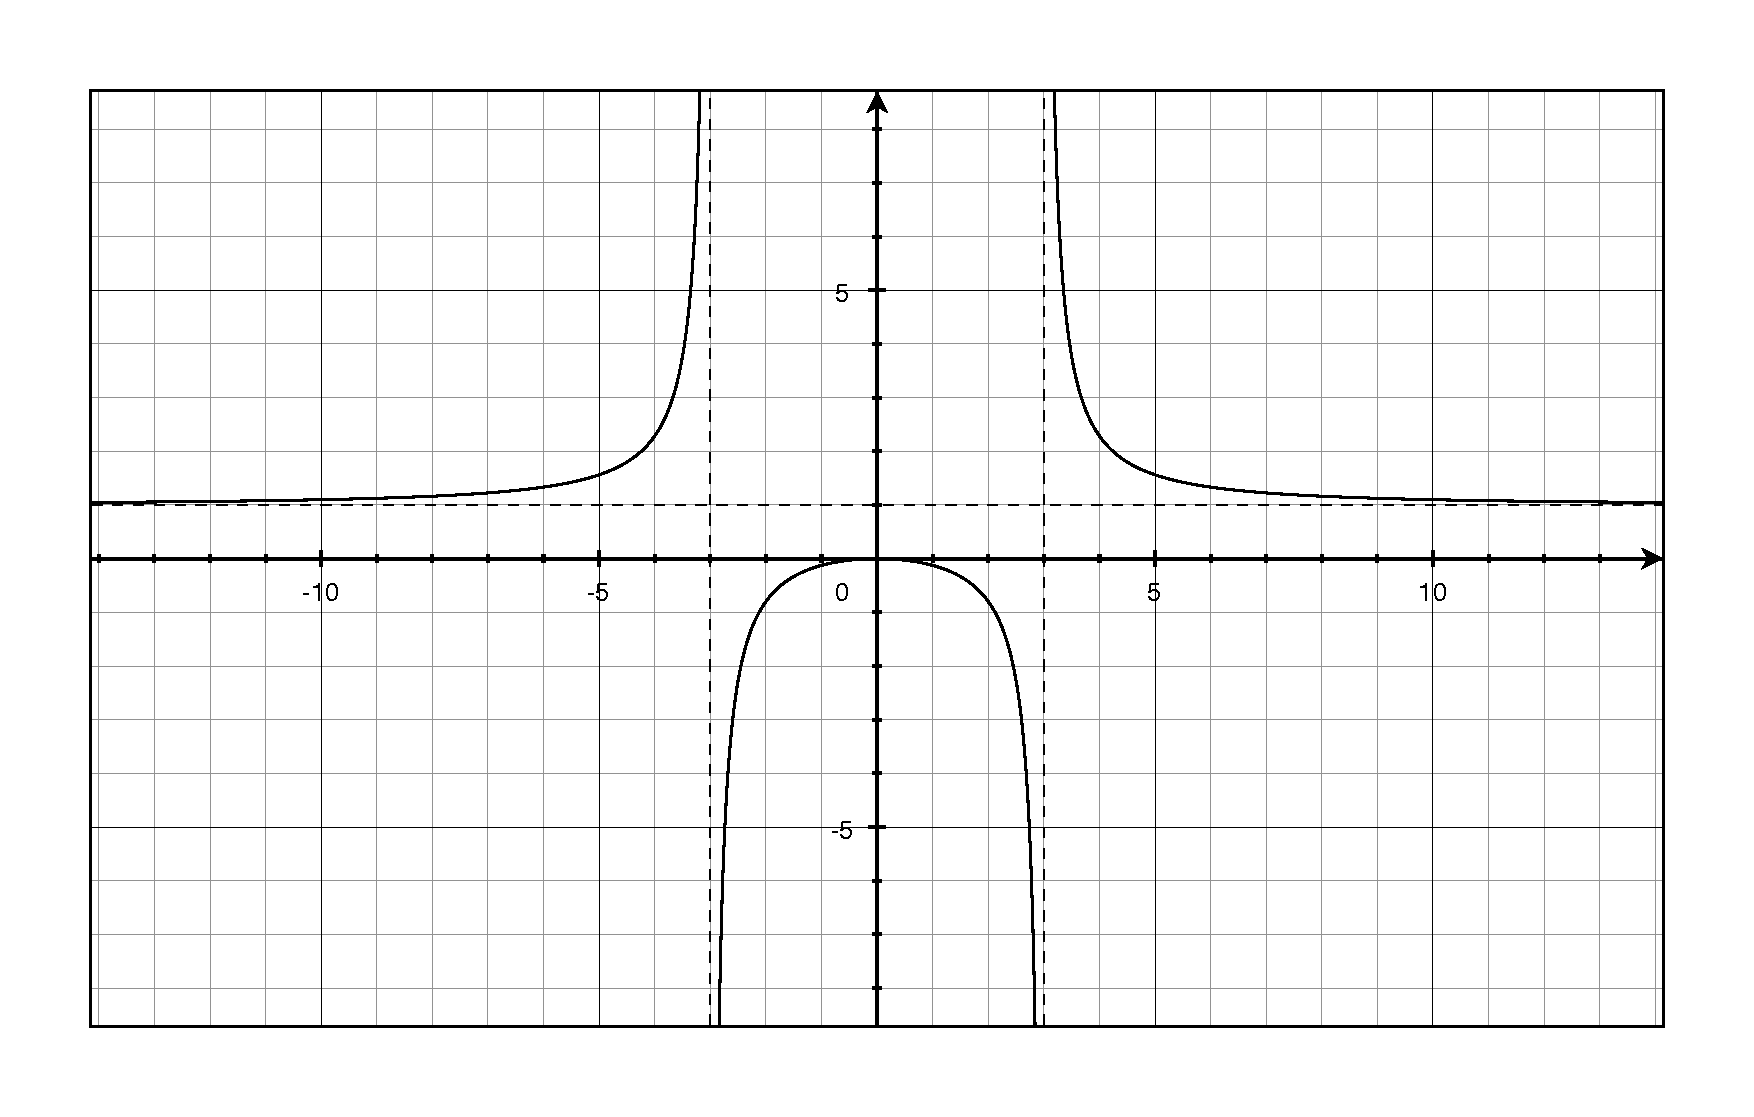
\includegraphics[width=12.25cm,height=8.75cm]{question35.eps}
  \caption*{Question 35}
\end{figure}

\item[36]
\begin{figure}[H]
  \centering
  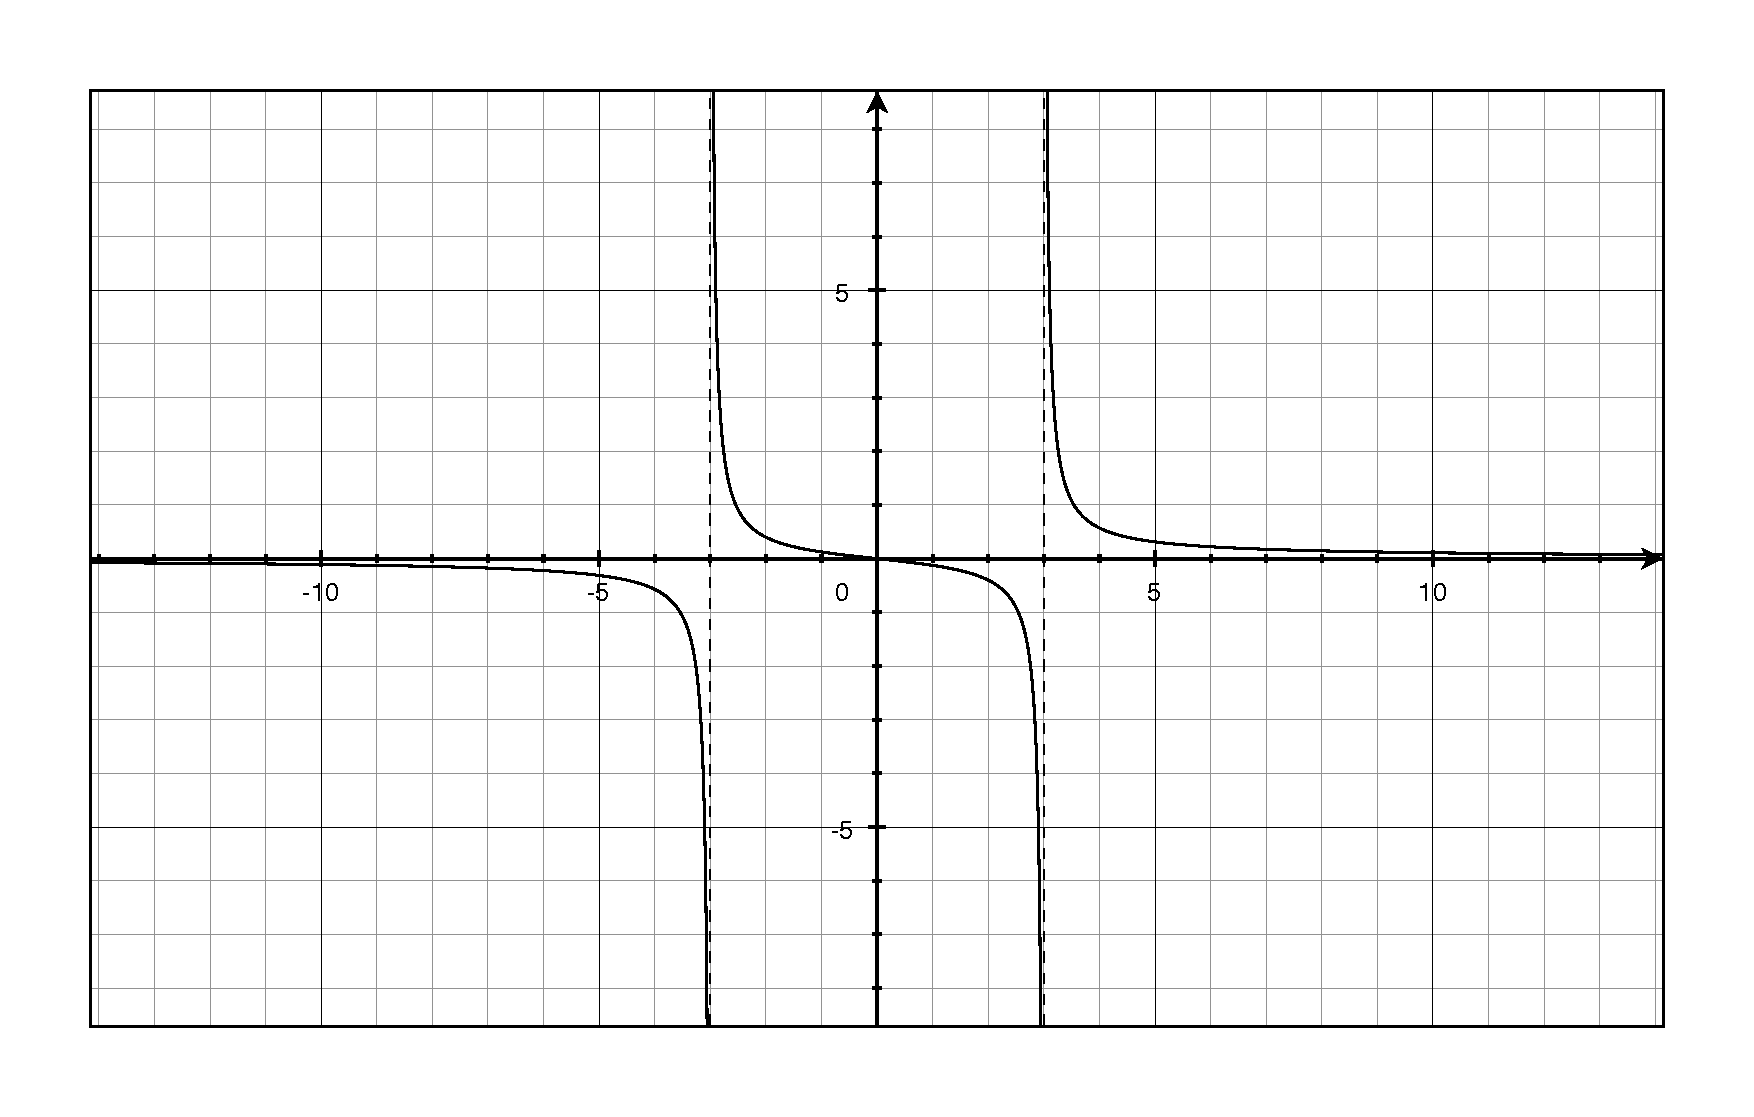
\includegraphics[width=12.25cm,height=8.75cm]{question36.eps}
  \caption*{Question 36}
\end{figure}

\item[39]
\begin{figure}[H]
  \centering
  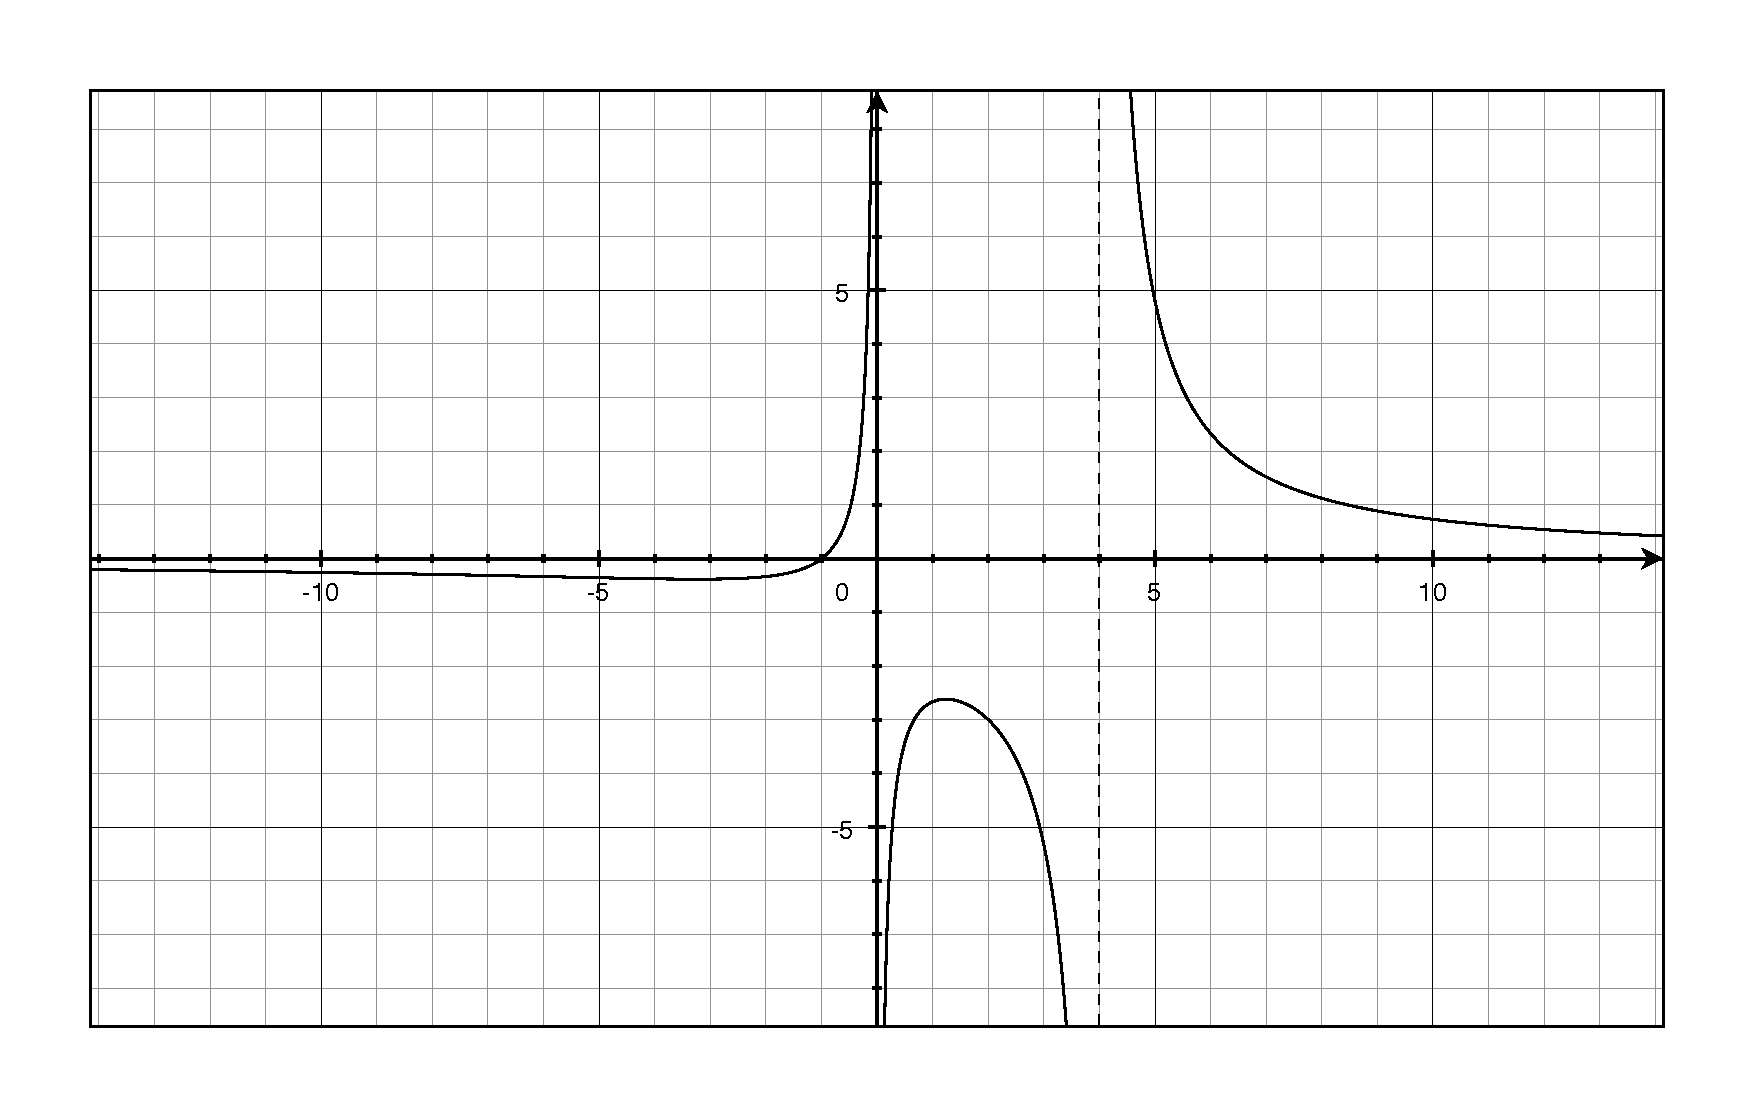
\includegraphics[width=12.25cm,height=8.75cm]{question39.eps}
  \caption*{Question 39}
\end{figure}

\item[40]
\begin{figure}[H]
  \centering
  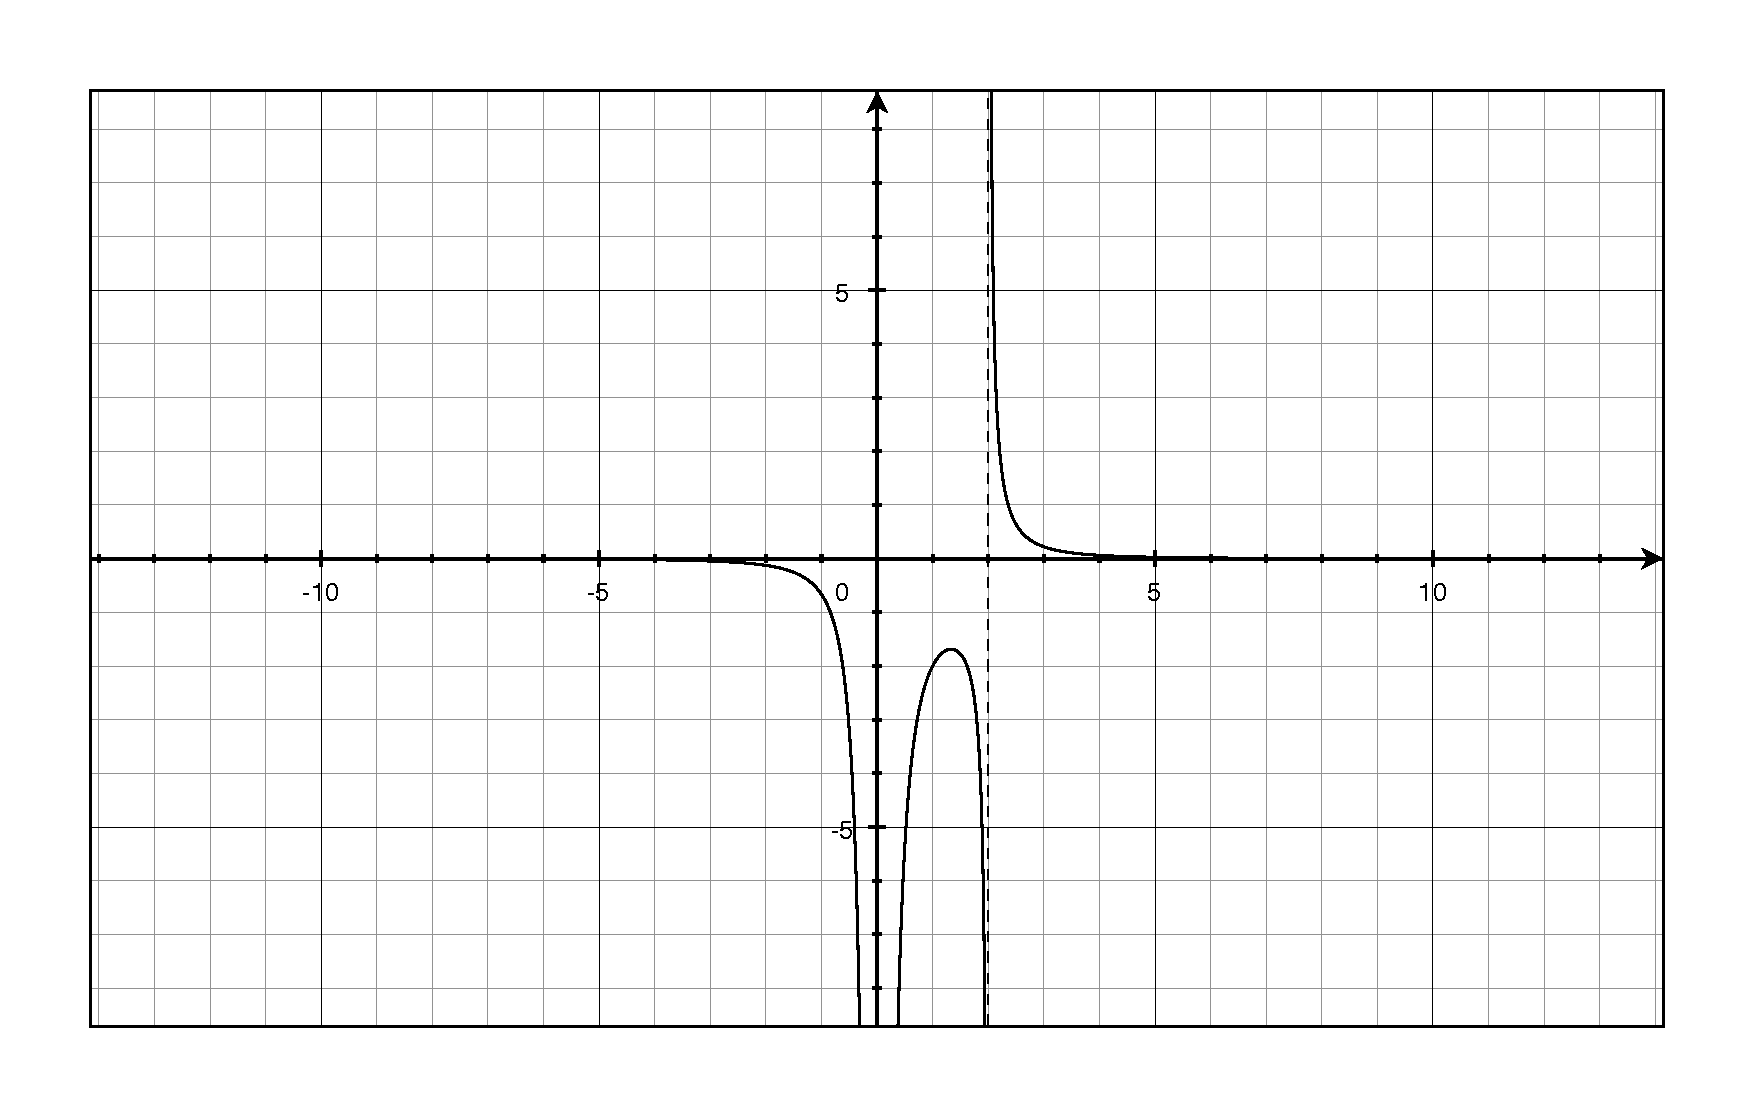
\includegraphics[width=12.25cm,height=8.75cm]{question40.eps}
  \caption*{Question 40}
\end{figure}

\item[44]
\begin{figure}[H]
  \centering
  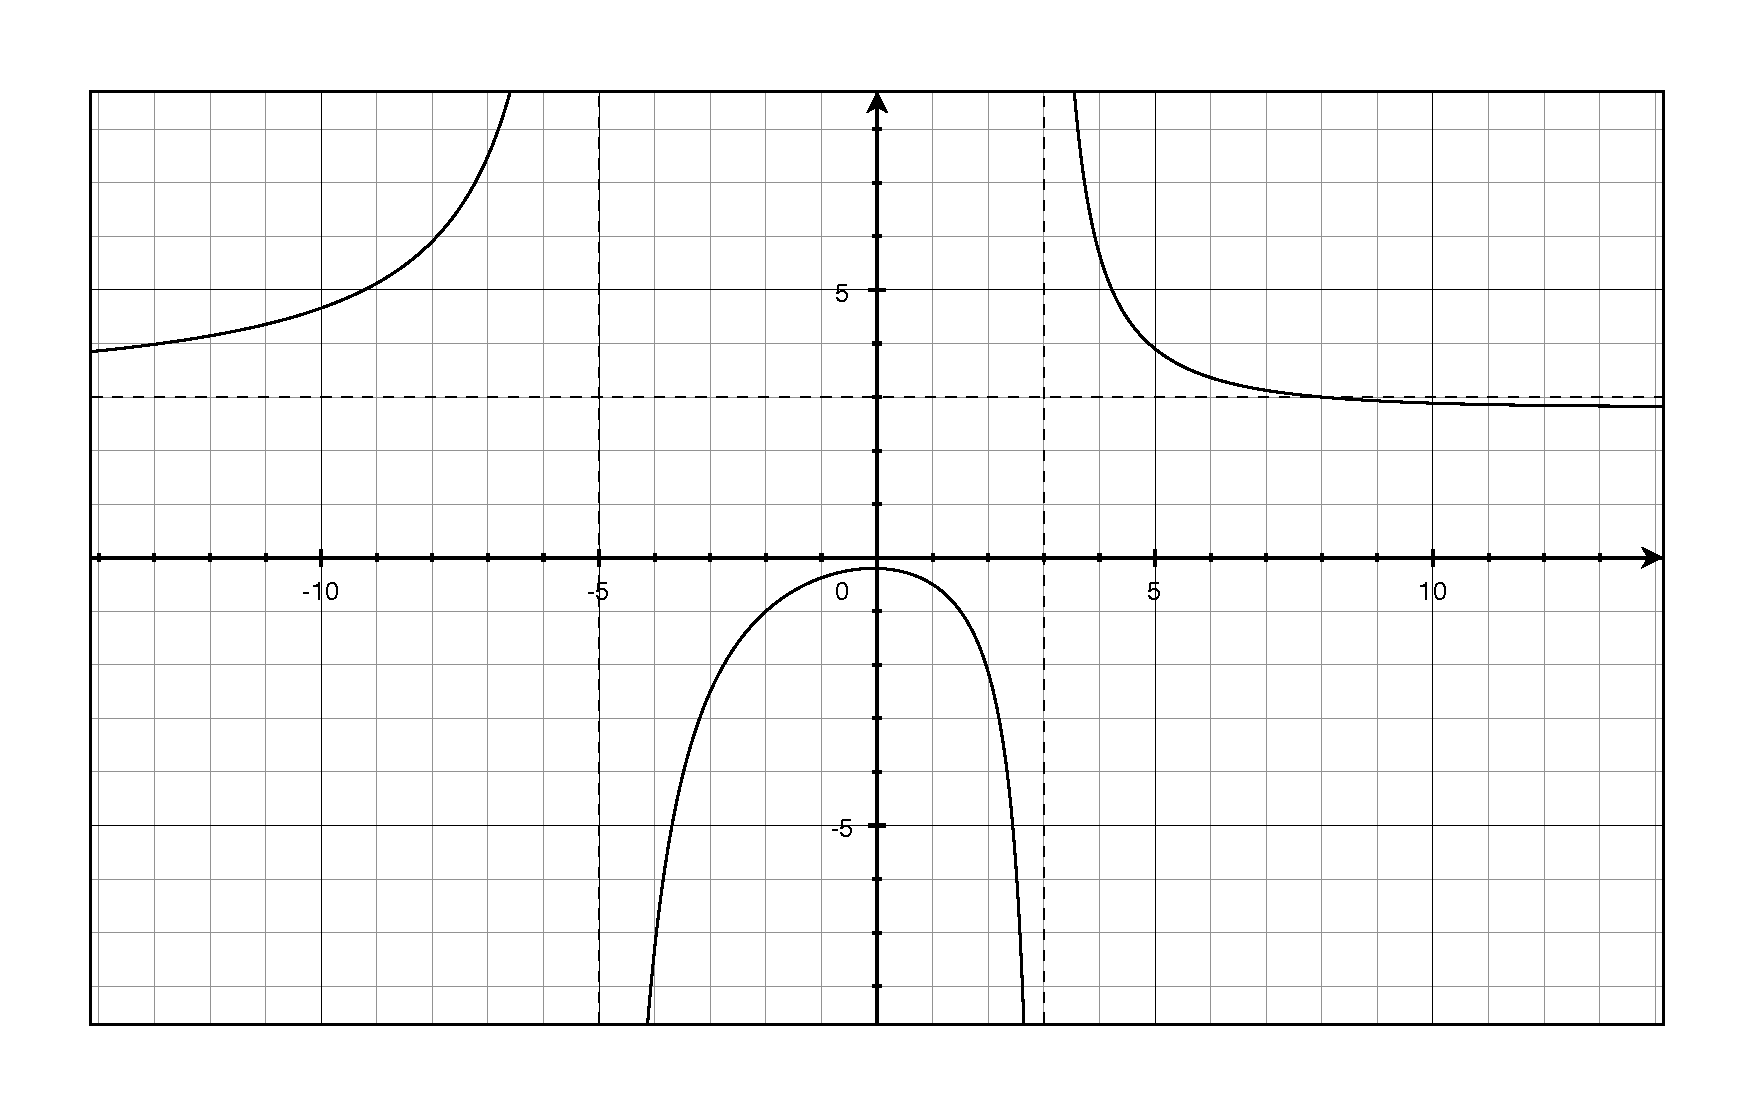
\includegraphics[width=12.25cm,height=8.75cm]{question44.eps}
  \caption*{Question 44}
\end{figure}

\item[53]
\begin{figure}[H]
  \centering
  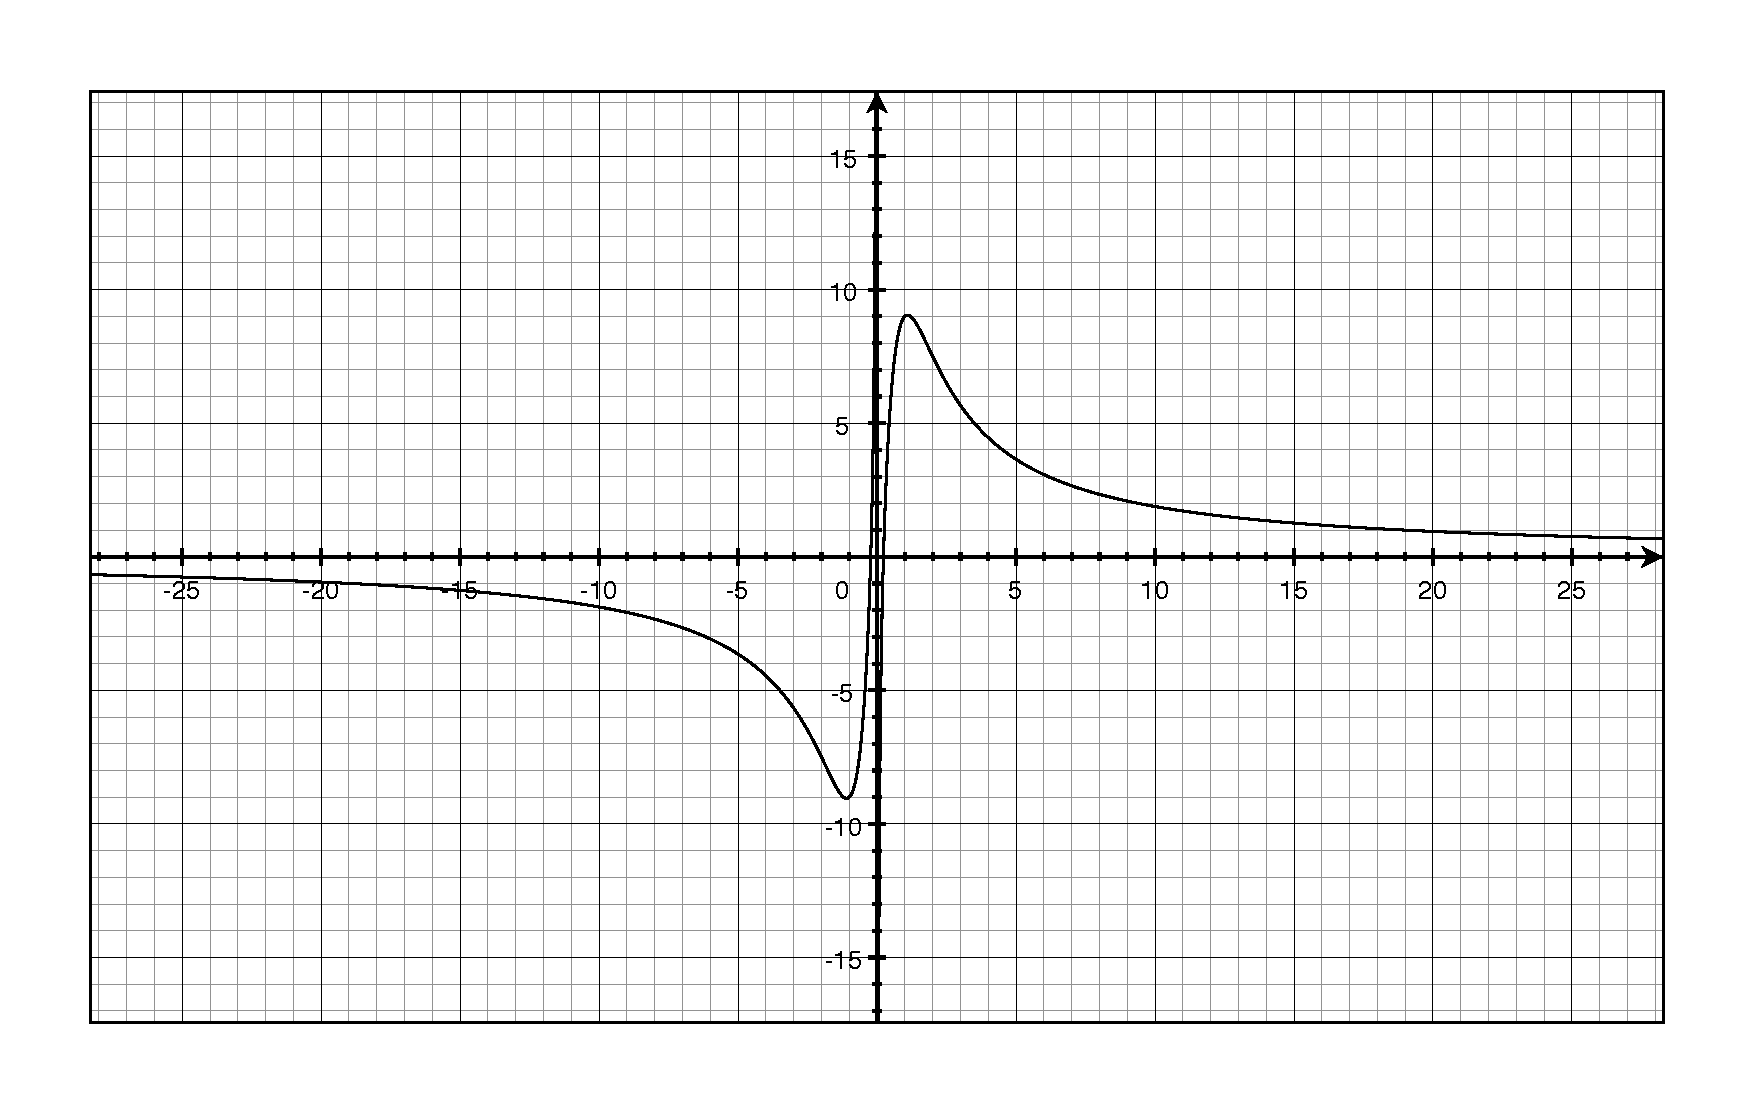
\includegraphics[width=12.25cm,height=8.75cm]{question53.eps}
  \caption*{Question 53}
\end{figure}

\item[55]
\begin{figure}[H]
  \centering
  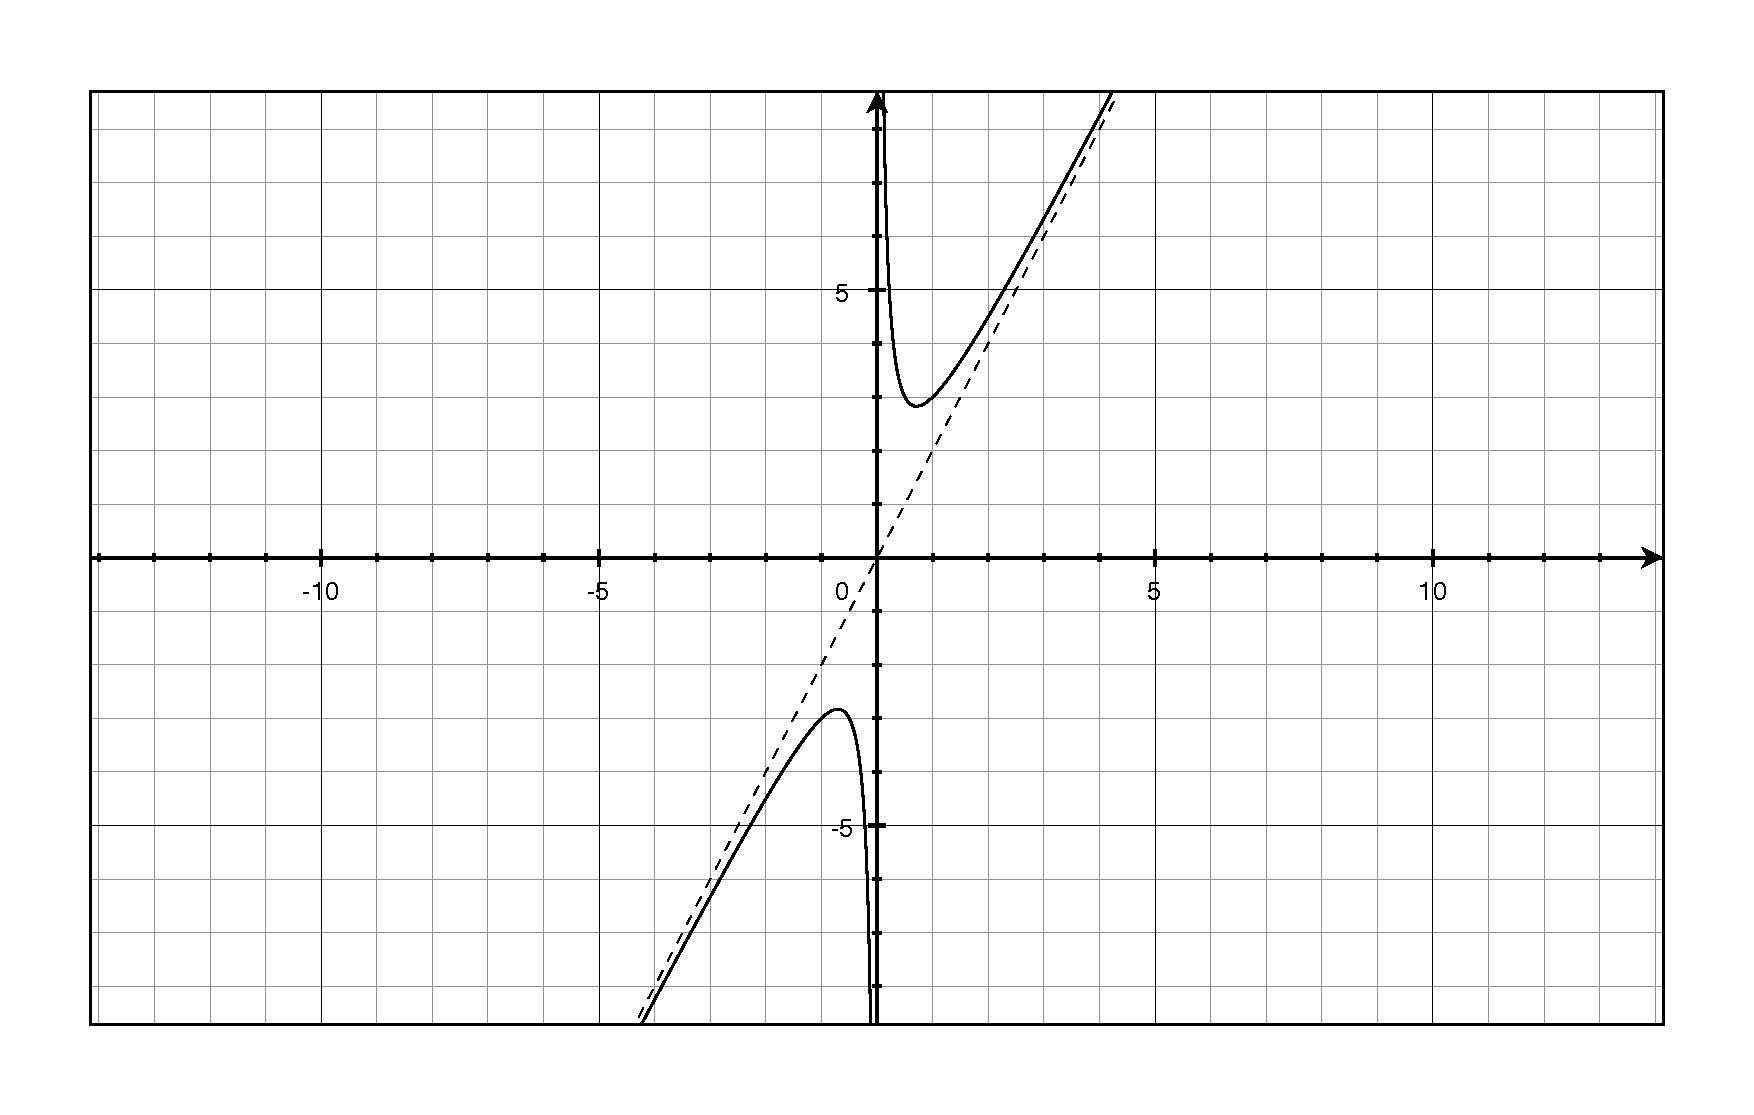
\includegraphics[width=12.25cm,height=8.75cm]{question55.eps}
  \caption*{Question 55}
\end{figure}

\item[56]
\begin{figure}[H]
  \centering
  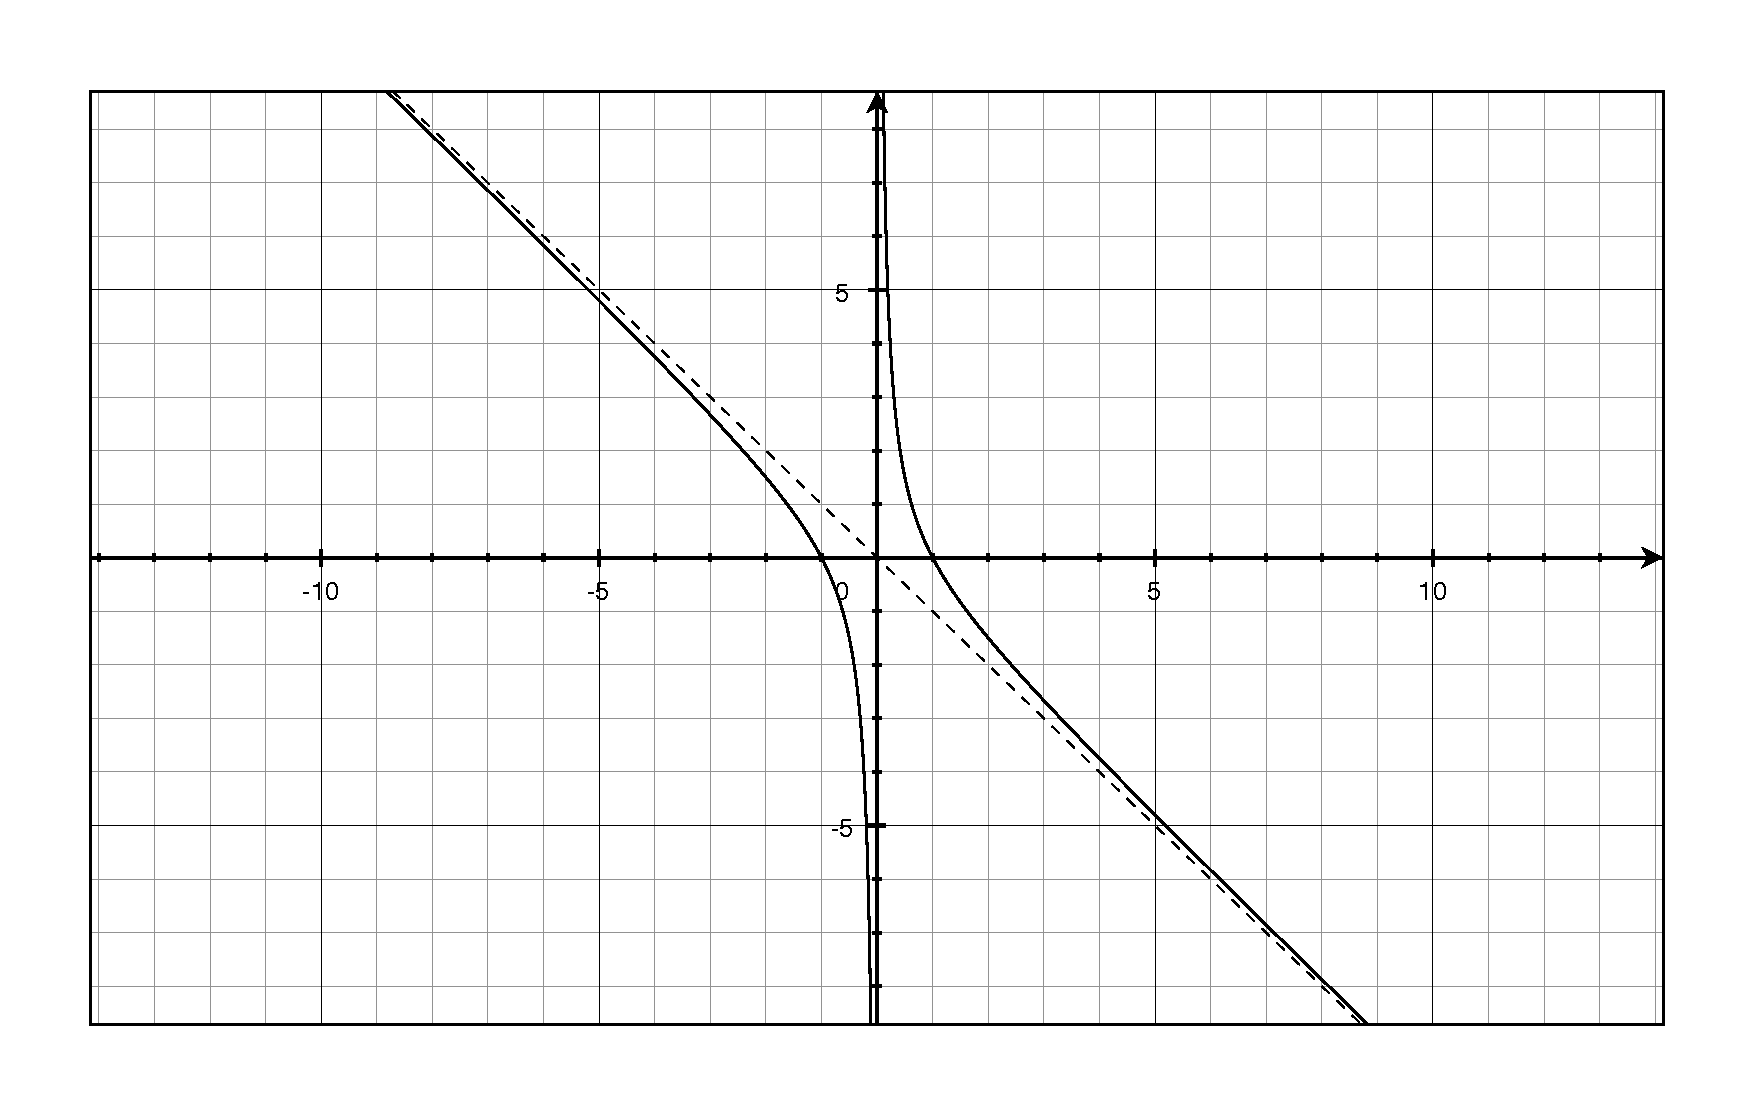
\includegraphics[width=12.25cm,height=8.75cm]{question56.eps}
  \caption*{Question 56}
\end{figure}

\item[61]
\begin{figure}[H]
  \centering
  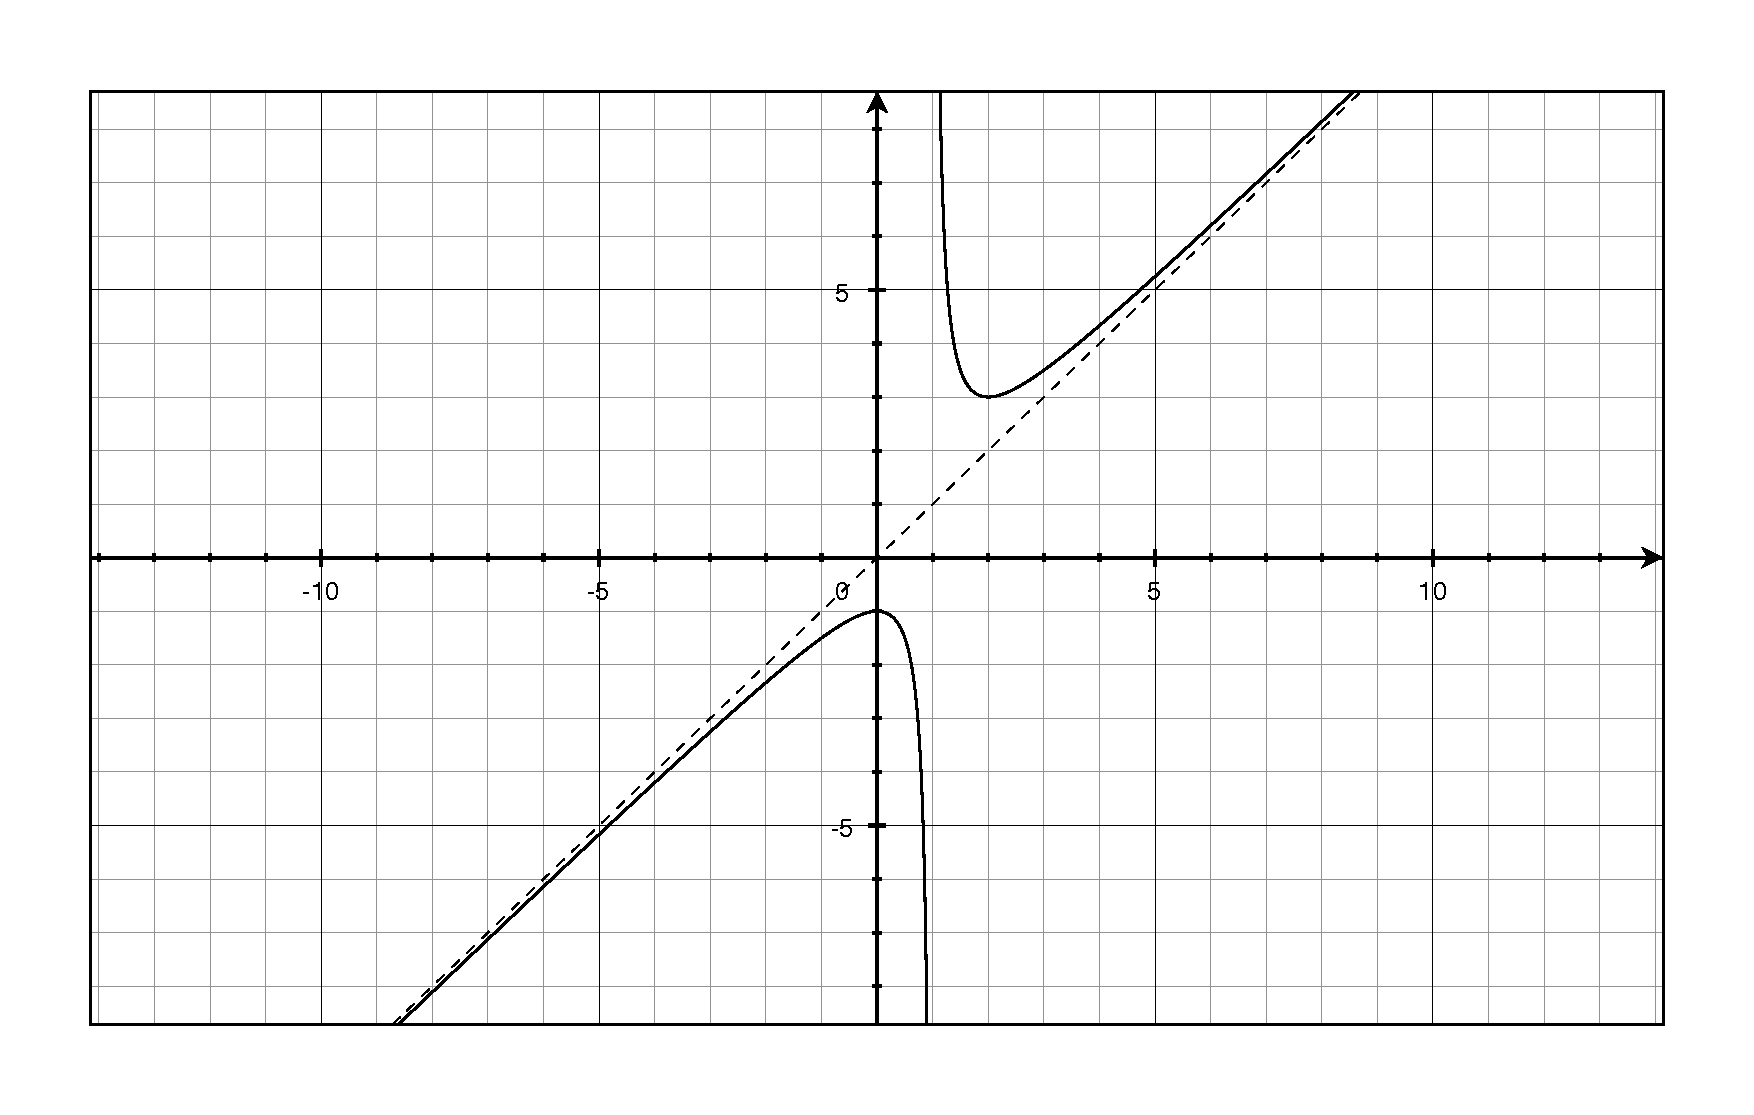
\includegraphics[width=12.25cm,height=8.75cm]{question61.eps}
  \caption*{Question 61}
\end{figure}

\item[62]
\begin{figure}[H]
  \centering
  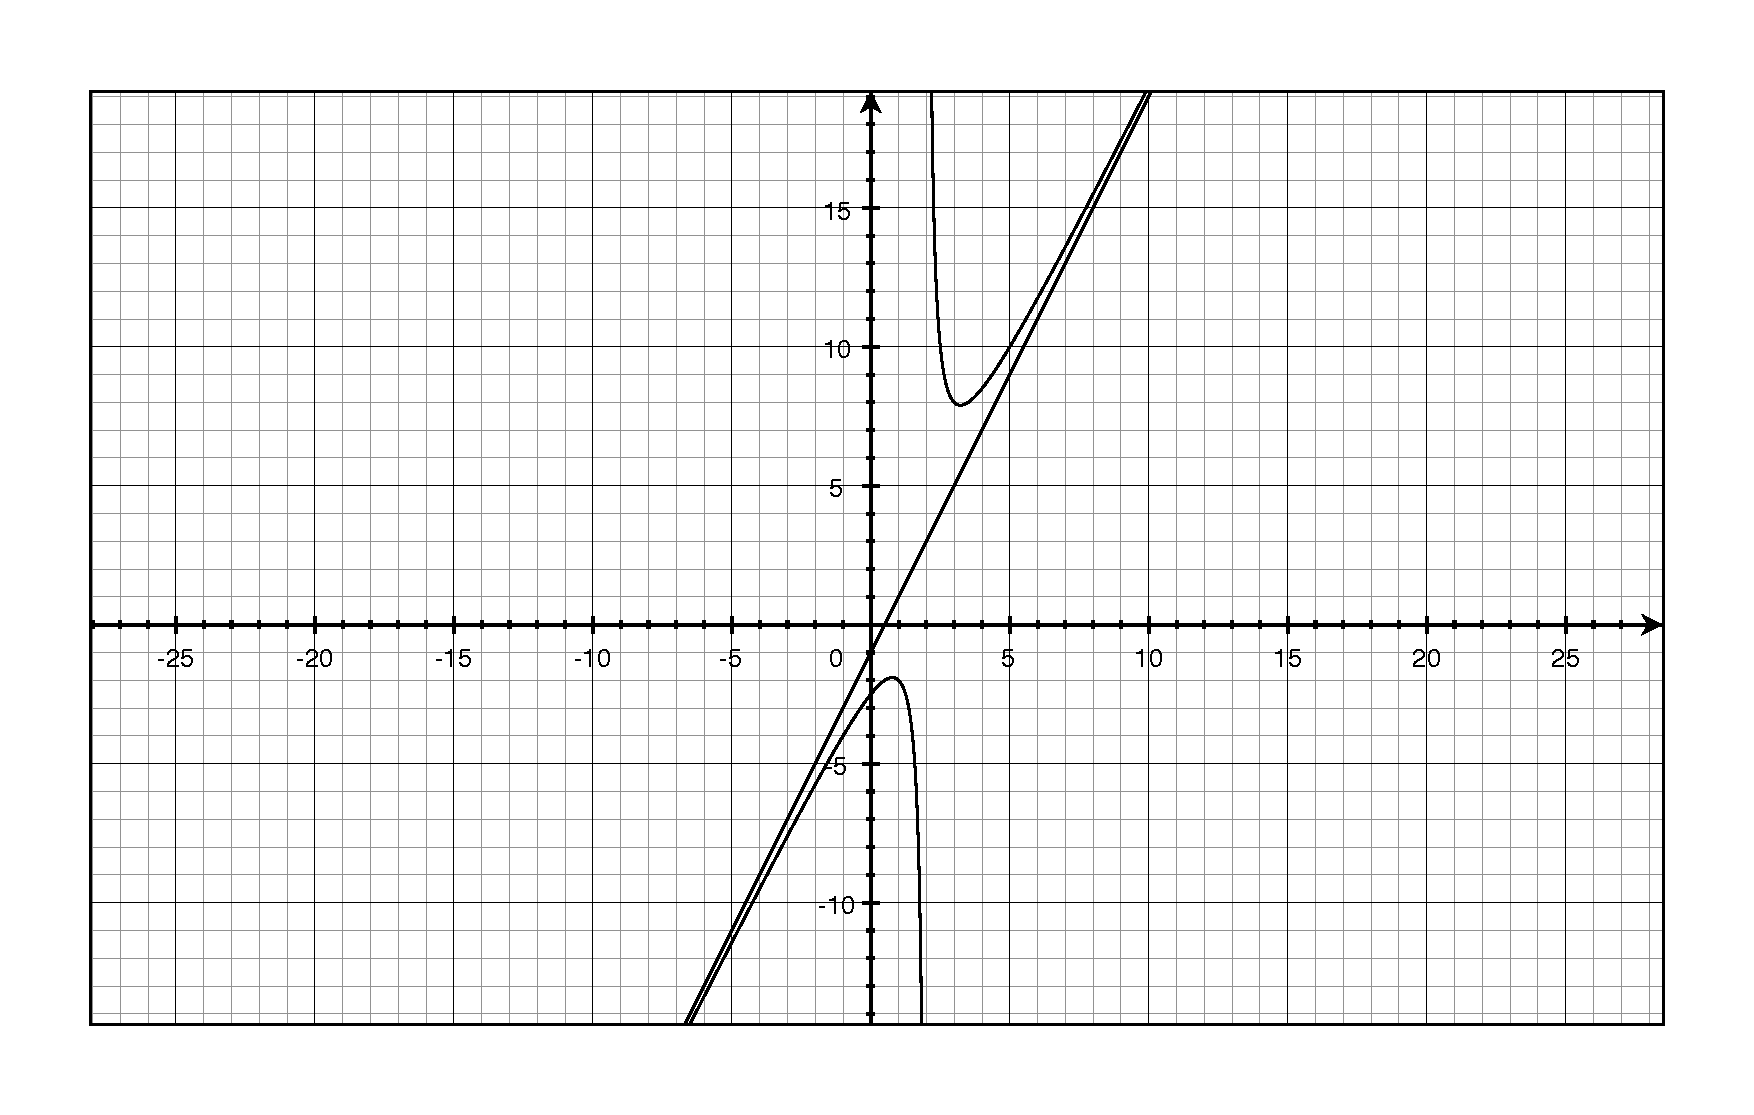
\includegraphics[width=12.25cm,height=8.75cm]{question62.eps}
  \caption*{Question 62}
\end{figure}

\item[71]
\[
  C(p) = \dfrac{255p}{100-p}
\]
\begin{description}

\item[a] $C(10) = 28.3$
\item[b] $C(40) = 170$
\item[c] $C(90) = 765$
\item[d] Since there is a vertical asymptote at $x=100$, it wouldn't be possible to remove all of the pollutants.

\end{description}

\begin{figure}[H]
  \centering
  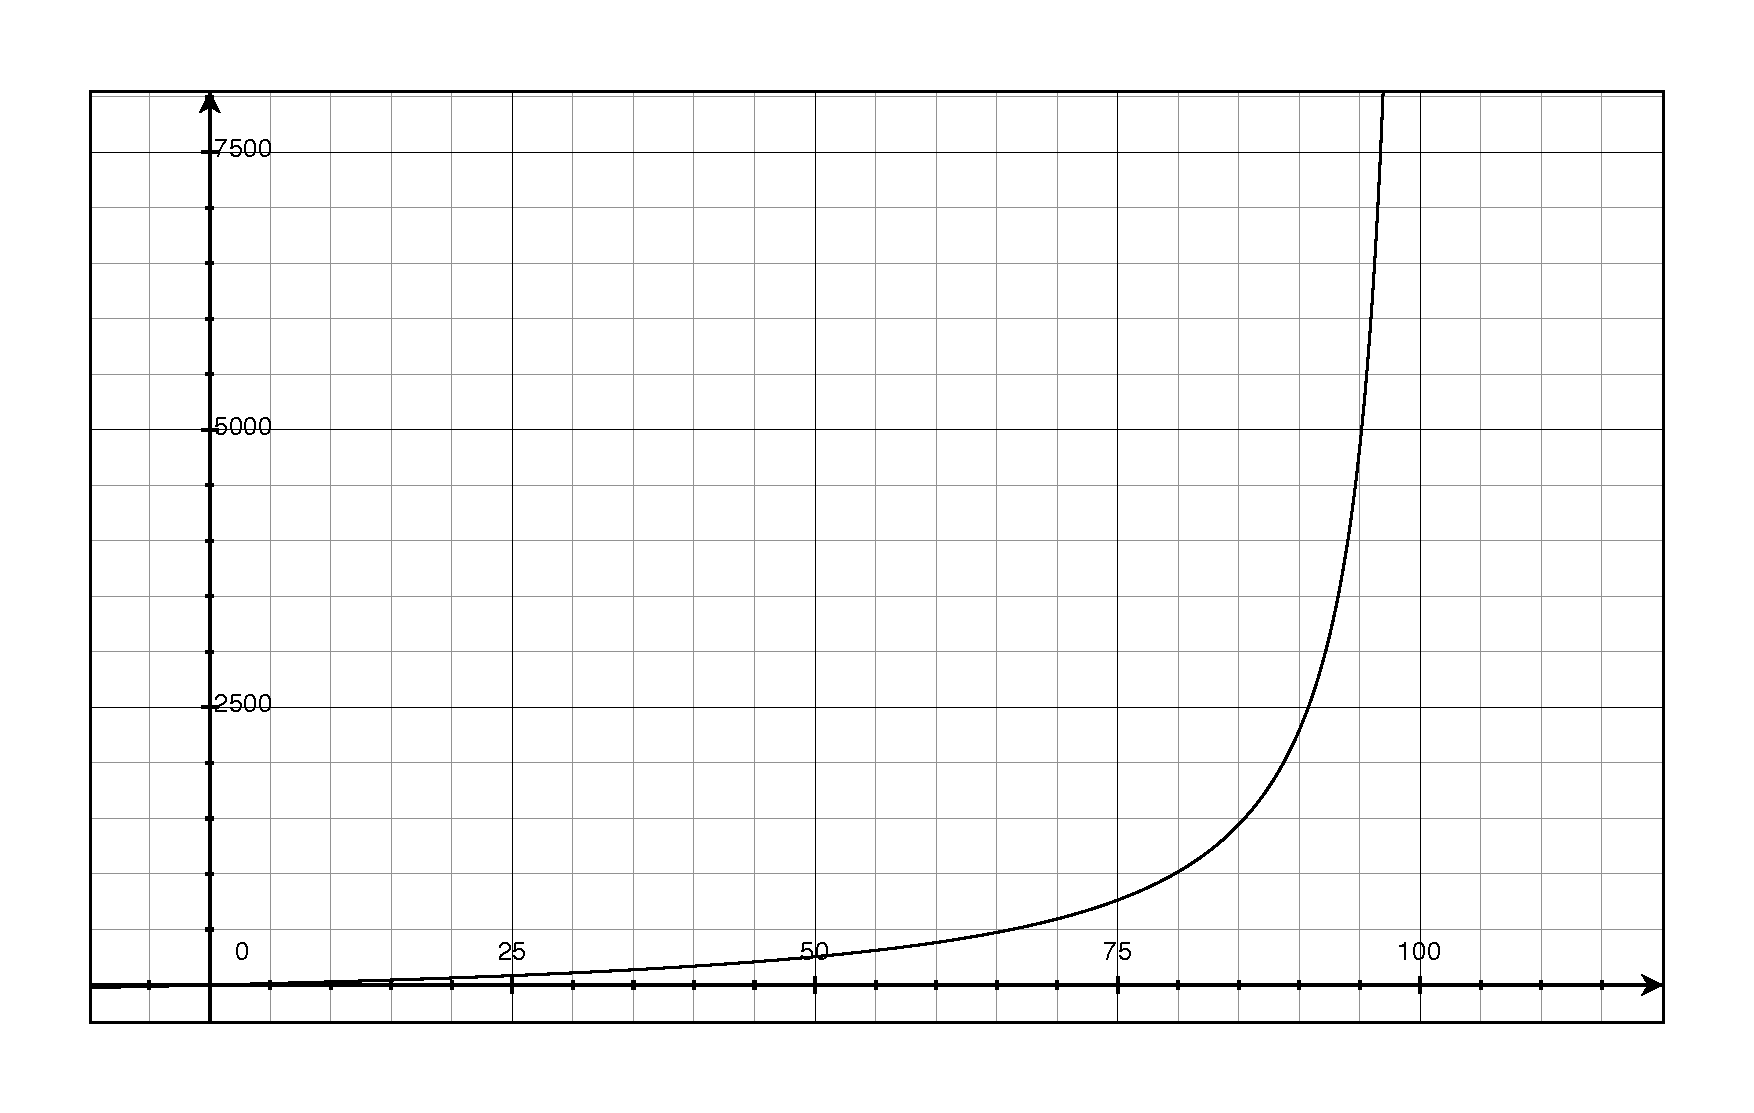
\includegraphics[width=12.25cm,height=8.75cm]{question71.eps}
  \caption*{Question 71}
\end{figure}

\pagebreak

\item[73]
\[
  N(t) = \dfrac{20(5+3t)}{1 + 0.04t}
\]

\begin{description}

\item[a] 
\begin{align*}
 N(5)  &= 333.3 \\
 N(10) &= 500 \\
 N(25) &= 800 \\
\end{align*}

\item[b]
We can re-write the equation to check for a horizontal asymptote:
\begin{align*}
  N(t) &= \dfrac{20(5+3t)}{1 + 0.04t} \\
       &= \dfrac{60t + 100}{0.04t + 1}
\end{align*}

So there is a horizontal asymptote at: $\dfrac{60}{0.04} = 1500$ and the herd will never be more than 1500 deer.

\end{description}

\begin{figure}[H]
  \centering
  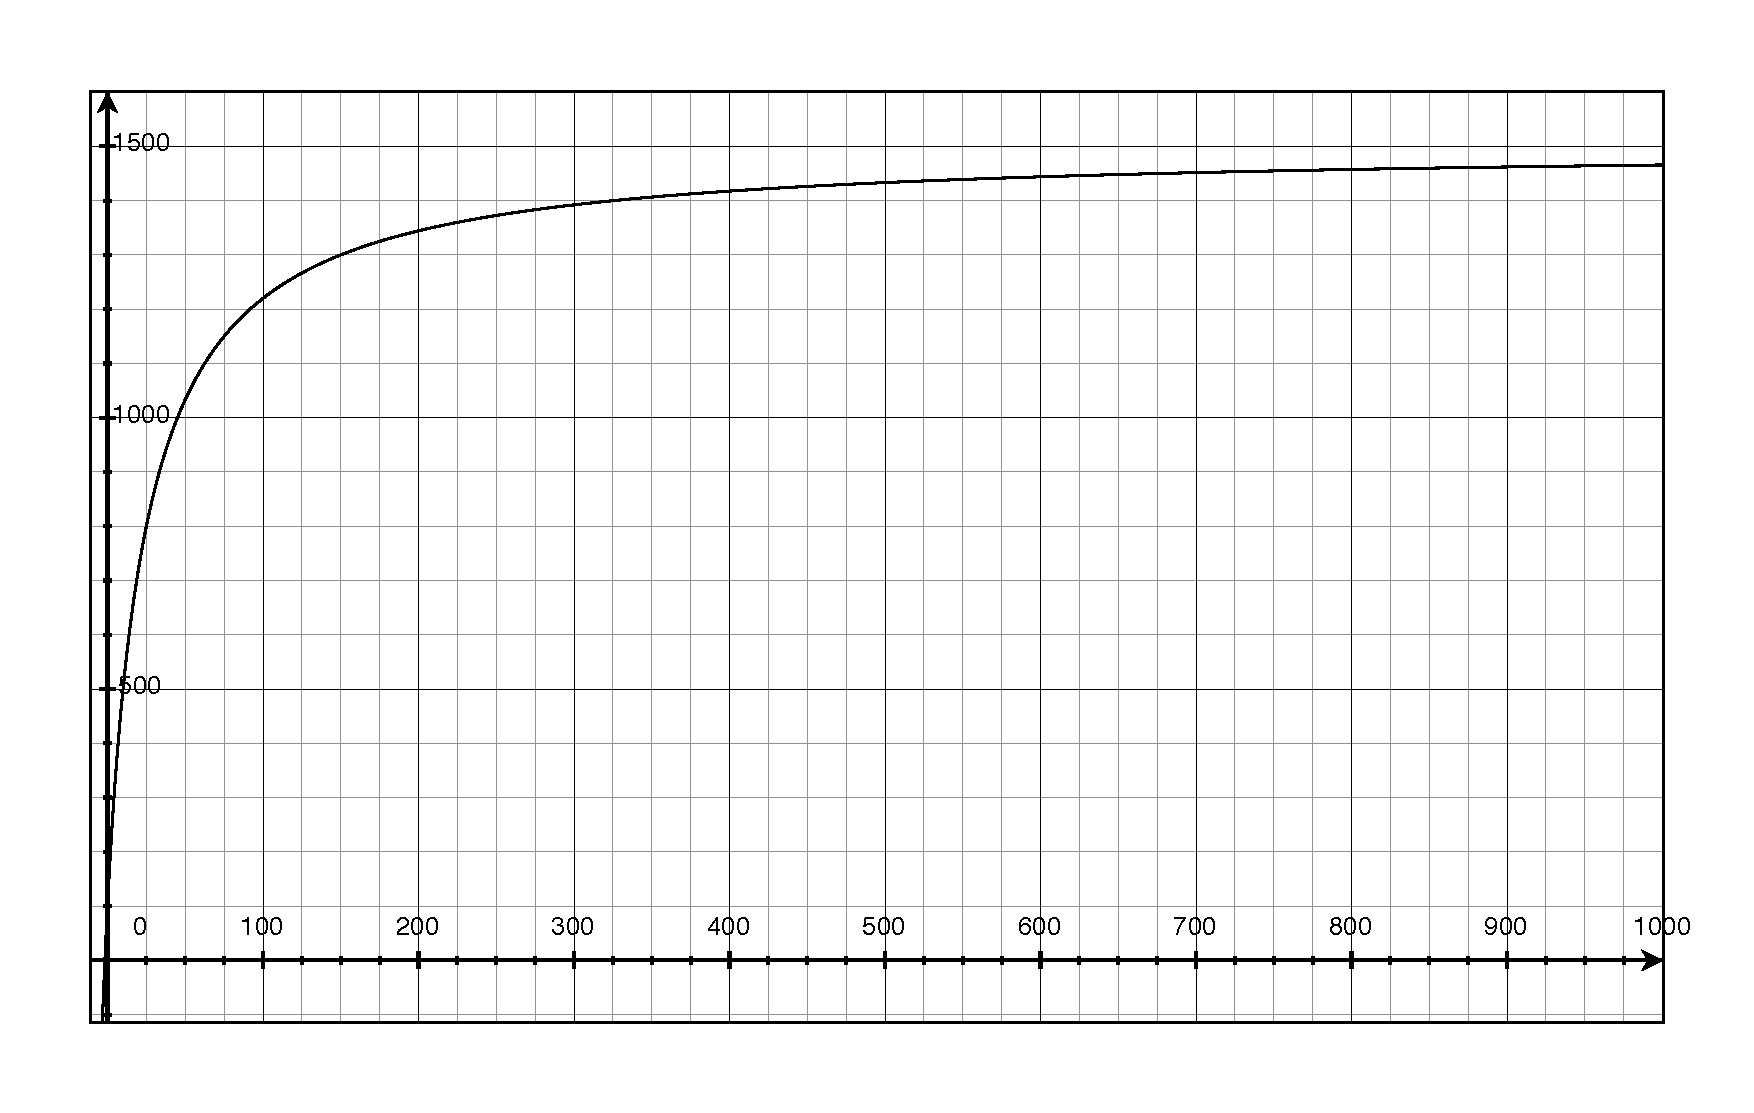
\includegraphics[width=12.25cm,height=8.75cm]{question73.eps}
  \caption*{Question 73}
\end{figure}

\end{description}

\fi

\pagebreak

\section{Extra Credit}

\begin{questions}

\question
Explain how you can tell that the function:
\[
  f(x) = \frac{x^6 + 10}{x^4 + 8x^2+15}
\]

has no x-intercept and no horizontal, vertical, or slant asymptote.

\begin{solution}
\begin{itemize}

\item From Descarte's {\em Rule of Signs}, $x^6+10$ has no positive or negative solutions, so there is no x-intercept.

\item From Descarte's {\em Rule of Signs}, $x^4+8x^2+15$ has no positive or negative solutions, so there are no vertical
  asymptotes.

\item Since the degree of the numerator is greater than the degree of the denominator, there is no horizontal asymptote.

\item Since the degree of the numerator is more than one greater than the degree of the denominator, there is no slant asymptote.

\end{itemize}

\end{solution}

\pagebreak

\question
Use long division and factoring to show that the function:
$f(x) = \dfrac{2x^2+4x+5}{x^2+2x+1}$

can be written as: $f(x) = 2 + \dfrac{3}{(x+1)^2}$

Then graph $f$ by transforming the graph of $y=\dfrac{1}{x^2}$

\begin{solution}
\[
\polylongdiv{2x^2+4x+5}{x^2+2x+1}
\]

\[
  f(x) = \frac{2x^2+4x+5}{x^2+2x+1} = 2 + \frac{3}{x^2+2x+1} = 2 + \frac{3}{(x+1)^2}
\]

The graph is the graph of $y=\dfrac{1}{x^2}$ scaled by 3, shifted up 2, and shifted left 1.
\end{solution}

\begin{figure}[H]
  \centering
  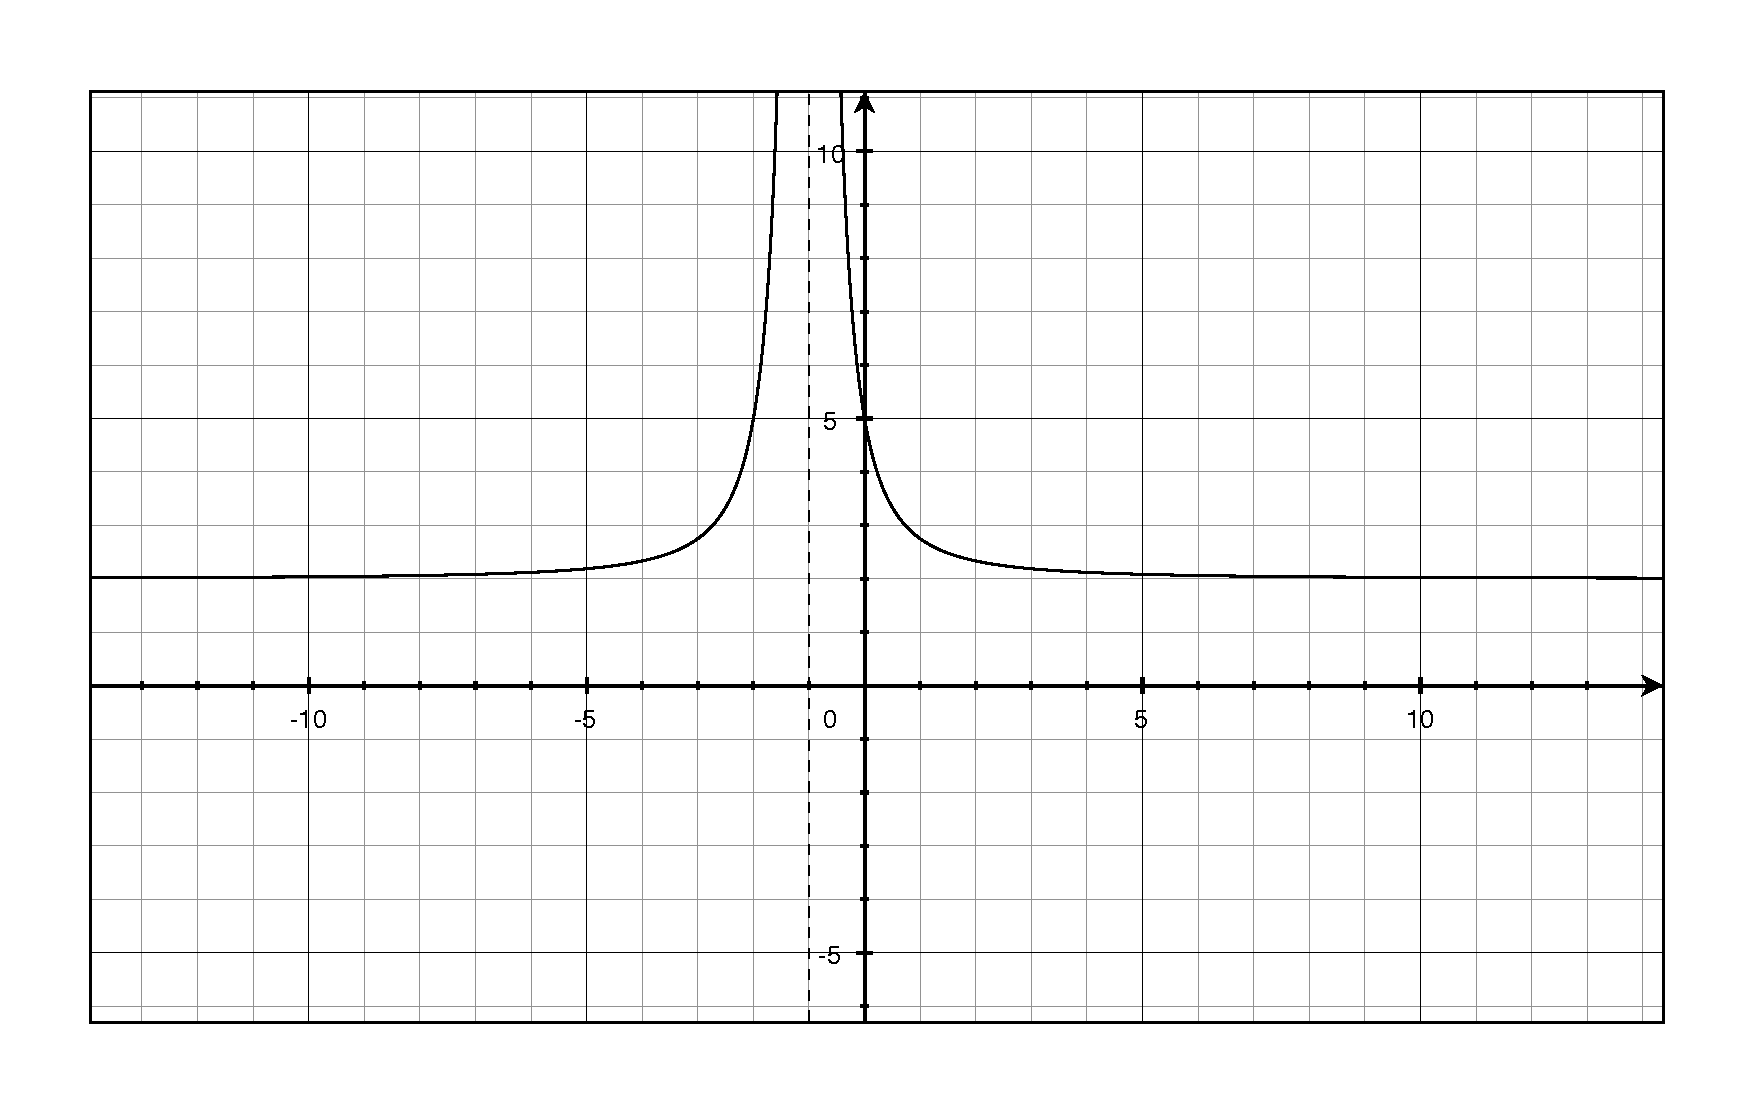
\includegraphics[width=12.25cm,height=8.75cm]{extra_credit.eps}
  \caption*{Extra Credit}
\end{figure}

\end{questions}

\ifprintanswers
\else
\vspace{1 cm}

{\em We will remember not the words of our enemies, but the silence of our friends.}
% {\em Injustice anywhere is a threat to justice everywhere.}
% {\em A nation that continues year after year to spend more money on military defense than on programs of social uplift
% is approaching spiritual doom.} 

\vspace{.1 cm}
\hspace{1 cm} --Martin Luther King

\fi

\end{document}

